\documentclass[titlepage]{article}

\usepackage[letterpaper,margin=1in,footskip=0.25in]{geometry}
\usepackage[nottoc,notlof,notlot]{tocbibind}
\usepackage[hidelinks]{hyperref}
\usepackage{fancyhdr}
\usepackage{subcaption}
\usepackage{tikz}
\usepackage{csquotes}
\usepackage{mdframed}
\usepackage{amssymb}
\usepackage{amsmath}
\usepackage{float}

\usetikzlibrary{knots,decorations.markings}

\colorlet{grx}{green!50!black}
\colorlet{pux}{red!50!blue}
\colorlet{gax}{black!50}
\colorlet{ylx}{yellow!70!black}
\colorlet{yly}{yellow!50!black}
\colorlet{ylz}{yellow!80!black}

\tikzset{
    verti/.style={gax,fill,inner sep=0pt,minimum width=1.6pt,minimum height=2mm},
    horiz/.style={gax,fill,inner sep=0pt,minimum width=2mm,minimum height=1.6pt}
}

\MakeOuterQuote{"}

\newmdenv[
    linewidth=0,
    backgroundcolor = blue!10,
    innertopmargin = \topskip,
    innerbottommargin = \topskip
]{defi}
\newmdenv[
    linewidth=0,
    backgroundcolor = yellow!80!red!10,
    innertopmargin = \topskip,
    innerbottommargin = \topskip
]{theor}
\newmdenv[
    linewidth=0,
    backgroundcolor = yellow!20!red!10,
    innertopmargin = \topskip,
    innerbottommargin = \topskip
]{conj}

\newcommand{\dq}[4][]{``#2"#1 \cite[#4]{#3}.}
\newcommand{\qed}{
    \begin{flushright}
        $\blacksquare$
    \end{flushright}
}

\title{Meditations on Bridge Number}
\author{Steven Labalme}
\date{\today}

\begin{document}




\pagenumbering{gobble}
\maketitle



\pagenumbering{roman}
\tableofcontents
\listoffigures
\listoftables
\newpage



\pagenumbering{arabic}
\pagestyle{fancy}
\fancyhf{}
\rfoot{Labalme \thepage}
\renewcommand{\headrulewidth}{0pt}
\begin{center}
    \setcounter{secnumdepth}{0}
    \section{Abstract}
    \setcounter{secnumdepth}{3}
\end{center}
Bridge number is a useful knot invariant for categorizing knots. More importantly, however, it appears in a number of places in knot theory and has been used in many proofs. Bridge number is interchangeably defined in two ways --- either (1) as the minimum number of maximal overpasses in any projection of the knot or (2) as the minimum number of unknotted, untangled arcs separated by a plane in any embedding of a knot in three-space (three-dimensional space). The second definition forms the basis of the standard method of determining bridge number, through a clever application of maxima and minima. This paper seeks to standardize the determination of bridge number using the first definition, revealing some curious and potentially powerful findings in the process.\par
This paper begins by defining bridge number and proving some of its properties, with a focus on alternating knots. The rest of the first section describes some important proofs that make use of bridge number. The second section concerns finding projections with the minimal number of bridges. The two simplest examples highlight some useful techniques and lay a framework through inductive reasoning and pattern recognition. With the success of certain techniques used in these examples, the paper gives formal definitions of these techniques and proves that they are valid. These strategies are then applied to a more complex problem to demonstrate their utility. In the last section, several conjectures are presented that provide a foundation for future research into the topics discussed herein.\par
Throughout this paper, important items will be placed in colored boxes. Blue boxes correspond to definitions, yellow boxes to theorems, and red boxes to conjectures. Please see \emph{The Knot Book: Notes} for additional background on any concepts throughout this paper \cite{bib:knotnotes}. Also see \emph{The Knot Book} by Colin C. Adams \cite{bib:knotbook}. This book will also be quoted on several occasions and paraphrased or summarized (sometimes without a direct reference) on other occasions.
\newpage



\section{Introduction to Bridge Number}
\subsection{Definitions and Elementary Properties}\label{sss:definitions}

\begin{figure}[h!]
    \centering
    \begin{subfigure}[b]{0.3\linewidth}
        \centering
        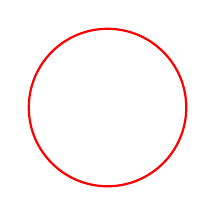
\begin{tikzpicture}
            \draw [red,thick] circle (1cm);
        \end{tikzpicture}
        \caption{The standard projection.}
        \label{fig:unknota}
    \end{subfigure}
    \begin{subfigure}[b]{0.3\linewidth}
        \centering
        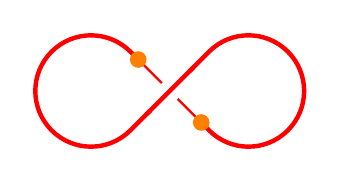
\begin{tikzpicture}
            \begin{knot}[
                clip width=5
            ]
                \strand[red,ultra thick] (-0.4,0.4)
                    to (-0.5,0.5)
                    arc [start angle=45,end angle=315,radius=0.707cm] (-0.5,-0.5)
                    to (0.5,0.5)
                    arc [start angle=135,end angle=-135,radius=0.707cm] (0.5,-0.5)
                    to (0.4,-0.4)
                ;
                \strand[red,thick] (-0.4,0.4) to (0.4,-0.4);
            \end{knot}
            \fill[orange] (-0.4,0.4) circle (3pt);
            \fill[orange] (0.4,-0.4) circle (3pt);
        \end{tikzpicture}
        \caption{A bridge projection.}
        \label{fig:unknotb}
    \end{subfigure}
    \begin{subfigure}[b]{0.3\linewidth}
        \centering
        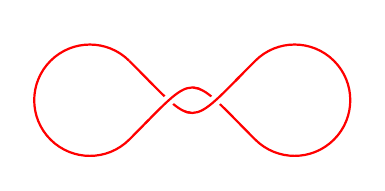
\begin{tikzpicture}
            \begin{knot}[
                clip width=5,
                consider self intersections,
                ignore endpoint intersections=false,
                flip crossing=1
            ]
                \strand[red,thick] (-0.8,0.5)
                    to [out=-45,in=-135,looseness=2] (0.8,0.5)
                    arc [start angle=135,end angle=-135,radius=0.707cm] (0.8,-0.5)
                    to [out=135,in=45,looseness=2] (-0.8,-0.5)
                    arc [start angle=315,end angle=45,radius=0.707cm]
                ;
            \end{knot}
        \end{tikzpicture}
        \caption{A two-bridge projection.}
        \label{fig:unknotc}
    \end{subfigure}
    \caption{The unknot projected three ways.}
    \label{fig:unknot}
\end{figure}

\noindent Although a knot, by definition, occupies three-dimensional space, knot theory often views them as two-dimensional projections. When the knot is "flattened" to draw a projection, knot theorists say that it lies in the projection plane. Even though crossings are inherently three-dimensional (one strand crossing over another necessitates depth), they are depicted such that the overstrand is continuous and the understrand is "broken," i.e., white space separates it from the overstrand. The idea of a projection allows for the development of knot invariants such as tricolorability. See Figure \ref{fig:unknotc} for a projection of the unknot obeying the normal rules of projections.\par
When considering bridge number, however, the knot is held to exist in overpasses and underpasses, which lie above and below the projection plane, respectively. These overpasses and underpasses are connected at their ends via vertices, which pass through the projection plane. In Figure \ref{fig:unknotb}, the thicker subarc is an overpass while the thinner subarc is an underpass$^[$\footnote{Note that the vertices' placement along the strand between crossings is entirely arbitrary, i.e., the understrand need not be substantially shorter than the overstrand, as depicted in Figure \ref{fig:unknotb}.}$^]$. They are connected at their ends by the orange vertices$^[$\footnote{Although most figures herein contain overpasses and underpasses, for simplicity's sake, not every subsequent projection will be drawn like Figure \ref{fig:unknotb} (with thicker and thinner strands and vertices).}$^]$.\par

\begin{figure}[h!]
    \centering
    \begin{subfigure}[b]{0.4\linewidth}
        \centering
        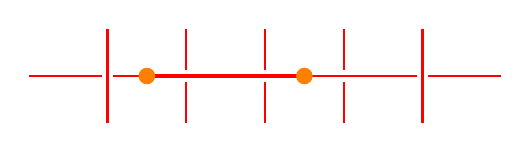
\begin{tikzpicture}
            \def\val{0.6}
            \begin{knot}[
                every strand/.append style={red,thick},
                clip width=5
            ]
                \strand (0,0) to (6,0);
                \strand (1,-\val) to (1,\val);
                \strand (2,-\val) to (2,\val);
                \strand (3,-\val) to (3,\val);
                \strand (4,-\val) to (4,\val);
                \strand (5,-\val) to (5,\val);
                \flipcrossings{1,5}
            \end{knot}
            \draw[red,ultra thick] (1.5,0) -- (3.5,0);
            \fill[orange] (1.5,0) circle (3pt);
            \fill[orange] (3.5,0) circle (3pt);
        \end{tikzpicture}
        \caption{An overpass.}
        \label{fig:overpassa}
    \end{subfigure}
    \begin{subfigure}[b]{0.4\linewidth}
        \centering
        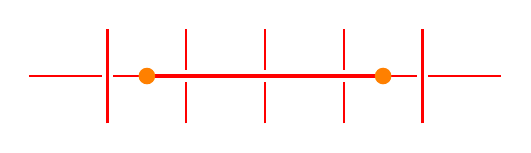
\begin{tikzpicture}[dot/.style={circle,fill=orange,outer sep=-1pt}]
            \def\val{0.6}
            \begin{knot}[
                every strand/.append style={red,thick},
                clip width=5
            ]
                \strand (0,0) to (6,0);
                \strand (1,-\val) to (1,\val);
                \strand (2,-\val) to (2,\val);
                \strand (3,-\val) to (3,\val);
                \strand (4,-\val) to (4,\val);
                \strand (5,-\val) to (5,\val);
                \flipcrossings{1,5}
            \end{knot}
            \draw[red,ultra thick] (1.5,0) -- (4.5,0);
            \fill[orange] (1.5,0) circle (3pt);
            \fill[orange] (4.5,0) circle (3pt);
        \end{tikzpicture}
        \caption{A maximal overpass.}
        \label{fig:overpassb}
    \end{subfigure}
    \caption{Overpasses.}
    \label{fig:overpass}
\end{figure}

In knots with multiple crossings, there may be some ambiguity as to what constitutes an overpass or underpass and to what extent. The following definitions and Figure \ref{fig:overpass} should clarify the concepts. Note that the inverse definitions hold for underpass, but since the theory of bridge number arbitrarily emphasizes overpasses, this paper will focus on overpasses, too.

\begin{defi}
    \begin{description}
        \item[Overpass] \hfill \\ \dq{A subarc of the knot that goes over at least one crossing but never goes under a crossing}{bib:knotbook}{64}
        \item[Maximal overpass] \hfill \\ \dq{An overpass that could not be made any longer}{bib:knotbook}{65}
    \end{description}
\end{defi}

Now that the foundations of bridge number have been introduced, bridge number will be defined as follows.

\begin{defi}
    \begin{description}
        \item[Bridge number] \hfill \\ \dq{The least number of unknotted arcs lying above the [projection] plane in any projection of the knot. \emph{Symbolically represented by} \textbf{\emph{b}(\emph{K})}}{bib:knotnotes}{25}
    \end{description}
\end{defi}

It is important to understand the difference between the \emph{bridge number} of a knot and the \emph{number of bridges} in a projection. Bridge number is a knot invariant, which means that is an inherent characteristic of a knot. It is a knot invariant because the least number of maximal overpasses in any projection of a knot obviously does not vary with the projection. The number of bridges, however, does vary with the projection, as it is the number of maximal overpasses in the projection at hand. For example, the number of bridges in Figure \ref{fig:unknotc} is 2 even though $b(K)=1$, as demonstrated by Figure \ref{fig:unknotb}$^[$\footnote{Note that knot theorists do say that the unknot has bridge number 1 (not 0) to avoid trivial exceptions despite the fact that a 0-crossing projection of the unknot exists. If it helps, think of the 0-crossing projection as resting entirely above the projection plane (hence being one single bridge).}$^]$.\par
Although bridge number and the number of bridges are quite different, the two work together to provide some simple bounds on a knot's bridge number. Two of these limits are defined below.

\begin{theor}
    \begin{description}
        \item[$b(K)\leq c(K)$] \hfill \\ \dq{The bridge number $b(K)$ of a nontrivial knot $K$ is always less than or equal to the least number of crossings in any projection of the knot}{bib:knotbook}{65}
        \item[$b(K)<c(K)$] \hfill \\ \dq{The bridge number $b(K)$ of a nontrivial knot $K$ is strictly less than the least number of crossings in any projection of the knot}{bib:knotbook}{65}
    \end{description}
\end{theor}

\paragraph{\textbf{Proof of 1}} For every knot $K$, there exists a projection with a minimal number of crossings, $c(K)$. Because each crossing must, by definition, have an overstrand and an understrand, there are $c(K)$ opportunities for distinct bridges. Thus, each crossing contributes at most one bridge to $b(K)$. Therefore, $b(K)$ cannot exceed $c(K)$.
\qed
\paragraph{\textbf{Proof of 2}} Consider alternating and nonalternating knots separately.

\begin{figure}[h!]
    \centering
    \begin{subfigure}[b]{0.3\linewidth}
        \centering
        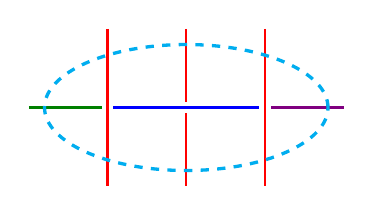
\begin{tikzpicture}
            \begin{knot}[
                every strand/.append style={thick},
                clip width=5,
                ignore endpoint intersections=false
            ]
                \strand[grx] (0,0) to (1,0);
                \strand[blue] (1,0) to (3,0);
                \strand[pux] (3,0) to (4,0);
                \strand[red] (1,1) to (1,-1);
                \strand[red] (2,1) to (2,-1);
                \strand[red] (3,1) to (3,-1);
                \flipcrossings{1,2,4,5}
            \end{knot}
            \draw[cyan,very thick,dashed] (2,0) ellipse (1.8cm and 0.8cm);
        \end{tikzpicture}
        \caption{A universal region.}
        \label{fig:2alterna}
    \end{subfigure}
    \begin{subfigure}[b]{0.3\linewidth}
        \centering
        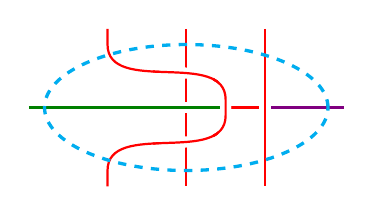
\begin{tikzpicture}
            \begin{knot}[
                every strand/.append style={thick},
                clip width=5,
                ignore endpoint intersections=false
            ]
                \strand[grx] (0,0) to (2.5,0);
                \strand[red] (2.5,0) to (3,0);
                \strand[pux] (3,0) to (4,0);
                \strand[red] (1,1)
                    to (1,0.8)
                    to [out=-90,in=90] (2.5,0.1)
                    to (2.5,-0.1)
                    to [out=-90,in=90] (1,-0.8)
                    to (1,-1)
                ;
                \strand[red] (2,1) to (2,-1);
                \strand[red] (3,1) to (3,-1);
                \flipcrossings{1,3,4,5}
            \end{knot}
            \draw[cyan,very thick,dashed] (2,0) ellipse (1.8cm and 0.8cm);
        \end{tikzpicture}
        \caption{A move.}
        \label{fig:2alternb}
    \end{subfigure}
    \caption{Combining two bridges in an alternating knot.}
    \label{fig:2altern}
\end{figure}

\subparagraph{\textbf{Alternating Knots}} For every alternating knot $K$, there exists a projection with its minimal number of crossings, $c(K)$. In this projection and by the definition of an alternating knot, sequential crossings will alternate (over, under, over, under, \dots). Because of this alternation and because $c(K)\geq 3$ for every alternating knot, there exists a region that can be drawn identical to Figure \ref{fig:2alterna}. In this region, there are three bridges that must be considered (\textcolor{grx}{green}, \textcolor{blue}{blue}, and \textcolor{pux}{purple}). The \textcolor{grx}{green} and \textcolor{blue}{blue} bridges will always be able to be combined by sliding the leftmost overstrand over the center understrand, as in Figure \ref{fig:2alternb}, reducing the number of bridges by 1. Note that although this move creates two new crossings, it creates no new bridges because the leftmost overstrand remains fully an overstrand and the middle understrand remains fully an understrand. Since at least 1 bridge can always be eliminated from the projection with $c(K)$ crossings (which originally has $c(K)$ bridges), $b(K)<c(K)$.
\subparagraph{\textbf{Nonalternating Knots}} For every nonalternating knot $K$, there exists a projection with its minimal number of crossings, $c(K)$. Because each crossing must, by definition, have an overstrand and an understrand, there are $c(K)$ opportunities for distinct bridges. However, since a nonalternating knot must, by definition, have at least one sequence of consecutive overstrands (and a matching sequence of consecutive understrands), at least one overpass and one underpass will span more than one crossing. Thus, at least two crossings must contribute to the same bridge at least once in a nonalternating knot. Therefore, $b(K)\leq c(K)-1\Rightarrow b(K)<c(K)$.
\qed

The previous two theorems together provide upper bounds on the bridge number of a nontrivial knot. In addition to them, there exists a lower bound on the bridge number of a nontrivial knot, as demonstrated by the theorem and proof below.

\begin{theor}
    \dq{If a knot has bridge number 1, it must be the unknot}{bib:knotbook}{65}
\end{theor}

\paragraph{Proof} If a knot has $b(K)=1$, there exists an embedding of it with at most one subarc lying above the projection plane and at most one subarc lying below the projection plane. These subarcs must be connected via vertices at either end. Assume that the projection plane is the $xy$-plane --- the knot will be considered in three-space in this proof.\par
Choose one of the two vertices on the overpass and assign an orientation to the knot such that the next vertex encountered will be the one on the other end of the overpass. Assign the chosen vertex a $z$-value of $1$. Traversing the overpass, linearly decrease the $z$-value assigned to each point until arriving at the other vertex, which will be assigned a $z$-value of $0.1$. Assign a $z$-value of $-0.1$ to the vertex on the underpass corresponding to the $z=0.1$ vertex of the overpass. These two sides of the same vertex should be connected by a line. Traversing the underpass, linearly decrease the $z$-value assigned to each point until arriving at the other vertex, which will be assigned a $z$-value of $-1$. The $z=-1$ and $z=1$ vertices should be connected by a line. Viewed from the top, this will be exactly the same knot. However, owing to the constantly decreasing $z$-value, this knot will be a loop with no crossings when viewed from the side. From this side view, it is clear that the knot is a planar isotropy of the unknot (a distortion of Figure \ref{fig:unknota}), and, therefore, is the unknot.
\qed


\subsection{Applications}\label{sss:applications}
As a knot invariant, bridge number is useful in distinguishing knots. However, there are some arguably more important applications of it. For instance, it can be proven that every two-bridge knot (literally a knot for which $b(K)=2$) is a rational knot and vice versa. Because the two-bridge/rational knots are a very well understood class of knots, theorems that are suspected to hold true for all knots are often first proven to hold true for the two-bridge knots.\par
Furthermore, properties of bridge number have been used to imply greater results. When attempting to prove that all rational knots are prime, H. Schubert turned to bridge number. Instead of directly proving this fact, he proved the following.

\begin{equation*}
    b(K_1\#K_2) = b(K_1)+b(K_2)-1
\end{equation*}

Since a knot must have $b(K)\geq 2$ to be distinct from the unknot (see Section \ref{sss:bridging}), the lowest possible bridge numbers of two factor knots $K_1$ and $K_2$ are 2 and 2. Thus, by the above equation, $b(K)\geq 3$ for a composite knot. Since all rational knots have $b(K)=2$, no rational knot is composite. Therefore, all rational knots are prime.\par
Building off of this result, Claus Ernst and Dewitt Sumners discovered a lower bound on the number of distinct prime knots of $n$ crossings. They did this by finding the following lower bound on the number of distinct two-bridge knots of $n$ crossings.

\begin{equation*}
    \frac{2^{n-2}-1}{3}
\end{equation*}

In addition to primality, bridge number provides an upper bound on the minimal genus standardly embedded surface upon which a knot can be embedded without crossings. In other words, it can be proven that if an $n$-embeddable knot $K$ \dq[ $n\leq b(K)$]{can be placed on a genus $n$ standardly embedded surface without crossings [and] cannot be placed on any standardly embedded surface of lower genus without crossings,}{bib:knotbook}{114}\par
Lastly, the idea of bridges has been used independently of bridge number. For example, J. W. Alexander proved that every knot or link has a closed braid representation by placing an axis between the overpasses and underpasses of a specifically constructed version of a knot.
\newpage



\section{Finding Projections with the Minimal Number of Bridges}
\subsection{Assembling Empirical Evidence}\label{sss:evidence}
\subsubsection{The Killzone in the Trefoil Knot}

\begin{figure}[h!]
    \centering
    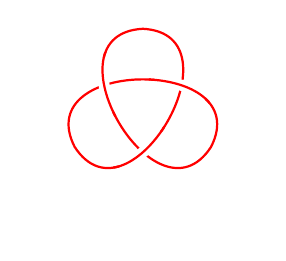
\begin{tikzpicture}
        \begin{knot}[
            clip width=5,
            consider self intersections
        ]
            \strand[red,thick] (90:1)
                \foreach \x in {1,2,3} {
                    to [bend left=117,looseness=1.9] ({90+120*\x}:1)
                }
            ;
            \flipcrossings{1,3}
        \end{knot}
    \end{tikzpicture}
    \vspace{-2.3em}
    \caption{The trefoil knot.}
    \label{fig:trefoil}
\end{figure}

\noindent When confronted with a standard projection of a knot, there are several immediate obstacles to reducing the number of bridges. Even with a knot as simple as the trefoil (Figure \ref{fig:trefoil}), the first issue may be its symmetry. Which of the three bridges should one try to eliminate since they're all the same shape, the same length, and in the same relative position? Eventually, the keen knot theorist may realize that this symmetry is not a roadblock; rather, it simply doesn't matter on which bridge one focuses.\par
However, there is a way to single out bridges for elimination. Many knots (the trefoil is no exception) are routinely drawn in loopy, symmetrical, aesthetically pleasing projections that obfuscate the mathematical relationship between crossings. Accordingly, redrawing a projection to concentrate crossings in an orderly fashion can reveal some of these relations. Fortunately, a simple method for doing so already exists: Dowker reconstructions.\par
When one reconstructs a knot projection from its Dowker notation (see \cite{bib:knotnotes}, Section 2.2), they create a line of crossings, each labeled with a Dowker pair. They will continue creating new crossings until they are forced to return to a previously drawn crossing. Thus, Dowker reconstructions often have every crossing in a rectangular region at the center of the projection while the strands connecting these crossings (which are not important in bridge number) loop around this region (see Figure \ref{fig:trefoilreconc}, which will subsequently be derived).\par

\begin{figure}[h!]
    \centering
    \begin{tikzpicture}
        \begin{knot}[
            clip width=5,
            consider self intersections
        ]
            \strand[red,thick,
            decoration={markings,
            mark=at position 0.2 with {\arrow{>}}},
            postaction={decorate}] (90:1)
                \foreach \x in {1,2,3} {
                    to [bend left=117,looseness=1.9] ({90+120*\x}:1)
                }
            ;
            \flipcrossings{1,3}
        \end{knot}
        \footnotesize
        \fill (30:0.57) circle (0pt)
            node[above right,xshift=-1pt,yshift=-1.5pt]{1}
            node[below left,yshift=2pt]{4}
        ;
        \fill (-90:0.57) circle (0pt)
            node[above,yshift=1pt]{2}
            node[below,yshift=-0.5pt]{5}
        ;
        \fill (150:0.57) circle (0pt)
            node[above right,xshift=-1.5pt,yshift=0.5pt]{3}
            node[below left,xshift=2pt,yshift=-0.5pt]{6}
        ;
    \end{tikzpicture}
    \vspace{-2.3em}
    \caption{The trefoil knot labeled in Dowker notation.}
    \label{fig:trefoilDowker}
\end{figure}

Let's find a Dowker reconstruction projection for the trefoil knot in Figure \ref{fig:trefoil}. Refer to Figure \ref{fig:trefoilDowker} throughout the following. Begin by assigning an orientation to the knot. Then arbitrarily choose a crossing (say, the upper-right one) and label it "1." Depart on the understrand and label every subsequent crossing with the next natural number until the original crossing is arrived at for the third time (do not label it with a third integer). At this point, each crossing has a pair of numbers, one even and one odd$^[$\footnote{This assertion can be proven.}$^]$.\par\par

\begin{table}[h!]
    \centering
    \begin{subtable}[b]{0.3\linewidth}
        \centering
        \begin{tabular}{ccc}
            4 & 6 & 2\\
            1 & 3 & 5
        \end{tabular}
        \caption{Dowker pairing.}
        \label{tab:trefoilDowkera}
    \end{subtable}
    \begin{subtable}[b]{0.3\linewidth}
        \centering
        \begin{tabular}{ccc}
            4 & 5 & 6\\
            1 & 2 & 3
        \end{tabular}
        \caption{Reconstruction pairing.}
        \label{tab:trefoilDowkerb}
    \end{subtable}
    \caption{Dowker pairs for the trefoil knot.}
    \label{tab:trefoilDowker}
\end{table}

Two versions of these pairings are shown in Table \ref{tab:trefoilDowker}. From the pairing in Table \ref{tab:trefoilDowkera}, it is possible to find the final Dowker notation (4 6 2). However, since a reconstructed projection is desired, Table \ref{tab:trefoilDowkerb} will be more useful.\par

\begin{figure}[h!]
    \centering
    \begin{subfigure}[b]{0.3\linewidth}
        \centering
        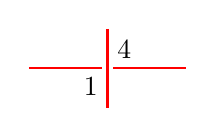
\begin{tikzpicture}
            \begin{knot}[
                every strand/.append style={red,thick},
                clip width=5
            ]
                \strand (0,0) to (2,0);
                \strand (1,0.5) to node[below left]{1}node[above right]{4}  (1,-0.5);
                \flipcrossings{1}
            \end{knot}
        \end{tikzpicture}
        \caption{1 crossing.}
        \label{fig:trefoilrecona}
    \end{subfigure}
    \begin{subfigure}[b]{0.3\linewidth}
        \centering
        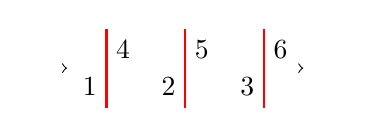
\begin{tikzpicture}
            \begin{knot}[
                every strand/.append style={red,thick},
                clip width=5
            ]
                \strand [decoration={markings,
                mark=at position 0.125 with {\arrow{>}},
                mark=at position 0.875 with {\arrow{>}}},
                postaction={decorate}] (0,0) to (4,0);
                \strand (1,0.5) to node[below left]{1}node[above right]{4}  (1,-0.5);
                \strand (2,0.5) to node[below left]{2}node[above right]{5}  (2,-0.5);
                \strand (3,0.5) to node[below left]{3}node[above right]{6}  (3,-0.5);
                \flipcrossings{1,3}
            \end{knot}
        \end{tikzpicture}
        \caption{3 crossings.}
        \label{fig:trefoilreconb}
    \end{subfigure}
    \begin{subfigure}[b]{0.3\linewidth}
        \centering
        \begin{tikzpicture}
            \begin{knot}[
                every strand/.append style={red,thick},
                clip width=5,
                consider self intersections
            ]
                \strand [decoration={markings,
                mark=at position 0.01 with {\arrow{>}},
                mark=at position 0.23 with {\arrow{>}}},
                postaction={decorate}] (0.5,0)
                    to (3.5,0)
                    to [out=0,in=-90] (4,0.5)
                    to [out=90,in=90] (1,0.5)
                    to node[below left]{1}node[above right]{4} (1,-0.5)
                    to [out=-90,in=-90] (2,-0.5)
                    to node[below left]{2}node[above right]{5} (2,0.5)
                    to [out=90,in=90] (3,0.5)
                    to node[below left]{3}node[above right]{6} (3,-0.5)
                    to [out=-90,in=-90] (0,-0.5)
                    to [out=90,in=180] cycle
                ;
                \flipcrossings{1,3}
            \end{knot}
        \end{tikzpicture}
        \vspace{-0.8em}
        \caption{Full reconstruction.}
        \label{fig:trefoilreconc}
    \end{subfigure}
    \caption{Reconstructing the trefoil knot from its Dowker notation.}
    \label{fig:trefoilrecon}
\end{figure}

Draw a crossing with a horizontal understrand and vertical overstrand, as in Figure \ref{fig:trefoilrecona}, and label it with the pair, 1 4. This is the first of three crossings to be drawn along the horizontal strand. The next two can either be drawn to the left or the right, so arbitrarily choose the right. Since this is an alternating knot, the crossings will alternate along the horizontal strand, as in Figure \ref{fig:trefoilreconb}. Also label the other crossings with their sequential pairs and assign the same orientation between the crossings as before. Notice how getting from crossing 1 to 2 requires leaving on the understrand, as was done in assigning the Dowker notation above. With the base strand drawn, continue through the rest of the crossings in numerical order, as in Figure \ref{fig:trefoilreconc}, before returning to the first crossing.\par

\begin{figure}[h!]
    \centering
    \begin{subfigure}[b]{0.3\linewidth}
        \centering
        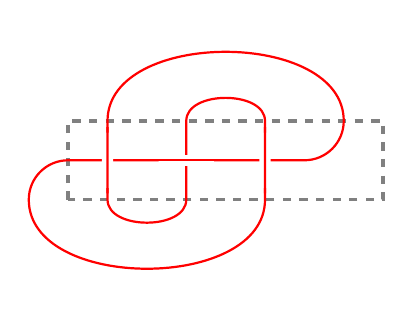
\begin{tikzpicture}
            \draw [gax,very thick,dashed] (0.5,-0.5) rectangle (4.5,0.5);
            \begin{knot}[
                clip width=5,
                consider self intersections
            ]
                \strand [red,thick] (0.5,0)
                    to (3.5,0)
                    to [out=0,in=-90] (4,0.5)
                    to [out=90,in=90] (1,0.5)
                    to (1,-0.5)
                    to [out=-90,in=-90] (2,-0.5)
                    to (2,0.5)
                    to [out=90,in=90] (3,0.5)
                    to (3,-0.5)
                    to [out=-90,in=-90] (0,-0.5)
                    to [out=90,in=180] cycle
                ;
                \flipcrossings{1,3}
            \end{knot}
        \end{tikzpicture}
        \vspace{-0.8em}
        \caption{The killzone's outline.}
        \label{fig:trefoilklzna}
    \end{subfigure}
    \begin{subfigure}[b]{0.3\linewidth}
        \centering
        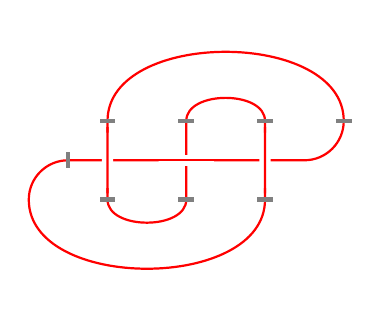
\begin{tikzpicture}
            \begin{knot}[
                clip width=5,
                consider self intersections
            ]
                \strand [red,thick] (0.5,0)
                    to (3.5,0)
                    to [out=0,in=-90] (4,0.5)
                    to [out=90,in=90] (1,0.5)
                    to (1,-0.5)
                    to [out=-90,in=-90] (2,-0.5)
                    to (2,0.5)
                    to [out=90,in=90] (3,0.5)
                    to (3,-0.5)
                    to [out=-90,in=-90] (0,-0.5)
                    to [out=90,in=180] cycle
                ;
                \flipcrossings{1,3}
            \end{knot}
            \node [verti] at (0.5,0) {};
            \node [horiz] at (4,0.5) {};
            \foreach \x in {1,2,3} {
                \foreach \y in {-0.5,0.5} {
                    \node [horiz] at (\x,\y) {};
                }
            }
        \end{tikzpicture}
        \vspace{-0.8em}
        \caption{Killzone notation.}
        \label{fig:trefoilklznb}
    \end{subfigure}
    \caption{The killzone in the trefoil knot.}
    \label{fig:trefoilklzn}
\end{figure}

The final reconstruction in Figure \ref{fig:trefoilreconc} is particularly useful because of the killzone, a region previously alluded to as motivation for drawing the Dowker reconstruction. This area is illustrated in Figure \ref{fig:trefoilklzn} and defined as follows.\par

\begin{defi}
    \begin{description}
        \item[Killzone] \hfill \\ The small region of a Dowker reconstruction that encloses all crossings in a rectilinear polygon; all crossings are arrayed along a grid.
    \end{description}
\end{defi}

Technically, the killzone is the boxed-in region in Figure \ref{fig:trefoilklzna}. However, to avoid drawing this every time, each strand is dashed where it enters and where it exits the killzone, as in Figure \ref{fig:trefoilklznb}. The importance of the killzone is that since bridge number directly deals with the relationship between crossings, moves that eliminate bridges can often be performed entirely within the killzone.


\subsubsection{Reducing the Number of Bridges in the Trefoil Knot}\label{ss2:trefoilreduce}
With the killzone providing an orderly arrangement of crossings (see Figure \ref{fig:trefoilklznb}), the issue of actually eliminating bridges arises. However, the solution can be found in the question, "how does one \emph{eliminate} a bridge?" Thinking about \emph{eliminating} bridges may lead to the thought process, "if the bridge going over crossing $x$ is the issue, how can I remove the crossing?" In a minimal-crossing projection, such as Figure \ref{fig:trefoilklznb}, obviously no crossing can be removed, and the budding knot theorist may become frustrated: "how can I remove bridges if I can't remove crossings?"\par
A simple change in wording can dramatically clarify the steps to reduce bridge number; instead of thinking about \emph{eliminating} bridges, think of \emph{combining} them. Search for ways to fuse two bridges by \emph{shifting} (not removing) the overstand(s) that separate(s) them.\par

\begin{figure}[h!]
    \centering
    \begin{subfigure}[b]{0.3\linewidth}
        \centering
        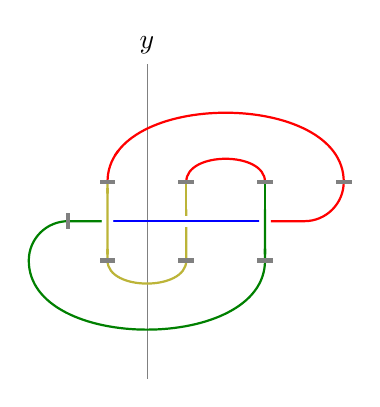
\begin{tikzpicture}
            \begin{knot}[
                clip width=5,
                consider self intersections,
                ignore endpoint intersections=false
            ]
                \draw [help lines] (1.5,-2) -- (1.5,2) node[above,black]{$y$};
                \strand [grx,thick] (3,0.5)
                    to (3,-0.5)
                    to [out=-90,in=-90] (0,-0.5)
                    to [out=90,in=180] (0.5,0)
                    to (1,0)
                ;
                \strand [blue,thick] (1,0) to (3,0);
                \strand [red,thick] (3,0)
                    to (3.5,0)
                    to [out=0,in=-90] (4,0.5)
                    to [out=90,in=90] (1,0.5)
                ;
                \strand [ylx,thick] (1,0.5)
                    to (1,-0.5)
                    to [out=-90,in=-90] (2,-0.5)
                    to (2,0.5)
                ;
                \strand [red,thick] (2,0.5) to [out=90,in=90] (3,0.5);
                \flipcrossings{4,5}
            \end{knot}
            \node [verti] at (0.5,0) {};
            \node [horiz] at (4,0.5) {};
            \foreach \x in {1,2,3} {
                \foreach \y in {-0.5,0.5} {
                    \node [horiz] at (\x,\y) {};
                }
            }
        \end{tikzpicture}
        \caption{3 bridges.}
        \label{fig:trefoilclra}
    \end{subfigure}
    \begin{subfigure}[b]{0.3\linewidth}
        \centering
        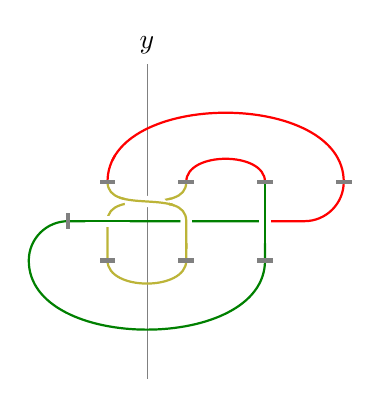
\begin{tikzpicture}
            \draw [help lines] (1.5,-2) -- (1.5,2) node[above,black]{$y$};
            \begin{knot}[
                clip width=5,
                clip radius=8pt,
                consider self intersections,
                ignore endpoint intersections=false
            ]
                \strand [grx,thick] (3,0.5)
                    to (3,-0.5)
                    to [out=-90,in=-90] (0,-0.5)
                    to [out=90,in=180] (0.5,0)
                    to (3,0)
                ;
                \strand [red,thick] (3,0)
                    to (3.5,0)
                    to [out=0,in=-90] (4,0.5)
                    to [out=90,in=90] (1,0.5)
                ;
                \strand [ylx,thick] (1,0.5)
                    to [out=-90,in=90] (2,0)
                    to (2,-0.5)
                    to [out=-90,in=-90] (1,-0.5)
                    to (1,0)
                    to [out=90,in=-90] (2,0.5)
                ;
                \strand [red,thick] (2,0.5) to [out=90,in=90] (3,0.5);
                \flipcrossings{4,5}
            \end{knot}
            \node [verti] at (0.5,0) {};
            \node [horiz] at (4,0.5) {};
            \foreach \x in {1,2,3} {
                \foreach \y in {-0.5,0.5} {
                    \node [horiz] at (\x,\y) {};
                }
            }
        \end{tikzpicture}
        \caption{2 bridges.}
        \label{fig:trefoilclrb}
    \end{subfigure}
    \caption{Combining bridges in the trefoil knot.}
    \label{fig:trefoilclr}
\end{figure}

Consider the \textcolor{grx}{green} and \textcolor{blue}{blue} bridges in Figure \ref{fig:trefoilclra}. What separates them is a segment of the third bridge (shaded \textcolor{ylx}{yellow} within the killzone). Now imagine this knot in three-space. Think of the left part of the \textcolor{ylx}{yellow} strand as depressing the \textcolor{grx}{green} and \textcolor{blue}{blue} bridges' connection through the projection plane while the right part of the \textcolor{ylx}{yellow} strand lifts the \textcolor{blue}{blue} bridge above the projection plane. If one "grabs" the curved part of the \textcolor{ylx}{yellow} bridge in their hand and rotates said hand $180^\circ$ clockwise about the $y$-axis while holding the ends of the \textcolor{ylx}{yellow} bridge steady, it could "flip" around, settling as in Figure \ref{fig:trefoilclrb}. Now the left part of the \textcolor{ylx}{yellow} strand lifts the corresponding part of the \textcolor{grx}{green} bridge above the projection plane while the right part depresses its corresponding bit through the projection plane. This will not alter any strand outside of the killzone (the \textcolor{ylx}{yellow} part outside simply changes to its mirror image) and will combine the \textcolor{grx}{green} and \textcolor{blue}{blue} bridges.\par

\begin{figure}[h!]
    \centering
    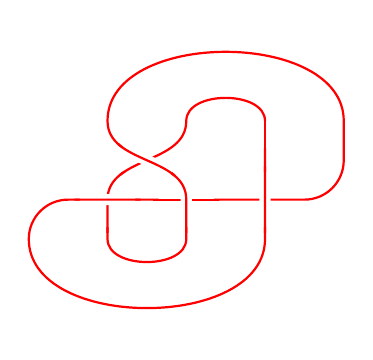
\begin{tikzpicture}
        \begin{knot}[
            clip width=5,
            consider self intersections,
            ignore endpoint intersections=false
        ]
            \strand [red,thick] (3,1)
                to (3,-0.5)
                to [out=-90,in=-90] (0,-0.5)
                to [out=90,in=180] (0.5,0)
                to (3.5,0)
                to [out=0,in=-90] (4,0.5)
                to (4,1)
                to [out=90,in=90] (1,1)
                to [out=-90,in=90] (2,0)
                to (2,-0.5)
                to [out=-90,in=-90] (1,-0.5)
                to (1,0)
                to [out=90,in=-90] (2,1)
                to [out=90,in=90] cycle;
            \flipcrossings{4,5}
        \end{knot}
    \end{tikzpicture}
    \vspace{-0.8em}
    \caption{A projection of the trefoil knot with 2 bridges.}
    \label{fig:trefoilfin}
\end{figure}

Because $b(3_1)=2$, Figure \ref{fig:trefoilclrb} is a minimal-bridge projection. This projection is cleaned up in Figure \ref{fig:trefoilfin}.


\subsubsection{The Ideal Killzone in the Figure-Eight Knot}

\begin{figure}[h!]
    \centering
    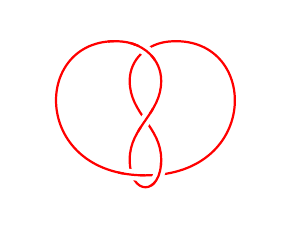
\begin{tikzpicture}
        \begin{knot}[
            clip width=5,
            clip radius=3pt,
            consider self intersections,
            ignore endpoint intersections=false
        ]
            \strand [red,thick] (-0.3,1)
                to [out=-5,in=90] (0.2,0.5)
                to [out=-90,in=90] (-0.2,-0.5)
                to [out=-90,in=-90,looseness=3] (0.2,-0.5)
                to [out=90,in=-90] (-0.2,0.5)
                to [out=90,in=-175] (0.3,1)
                to [out=5,in=0,out looseness=1.7,in looseness=2.2] (0,-0.7)
                to [out=180,in=175,out looseness=2.2,in looseness=1.7] cycle
            ;
            \flipcrossings{3,5}
        \end{knot}
    \end{tikzpicture}
    \vspace{-0.4em}
    \caption{The figure-eight knot.}
    \label{fig:fig8}
\end{figure}

\noindent To avoid redundancy, the progression from Figure \ref{fig:fig8} to its Dowker reconstruction will not be as painstakingly detailed as the previous one. However, it will be used to highlight an important fact about the killzone.\par
Before attacking the figure-eight knot, consider the labeling of the trefoil knot (Figure \ref{fig:trefoilDowker}). Note that there is only one way to Dowker-label the trefoil knot --- because of the symmetry of the trefoil, starting at any crossing with any orientation leads to the same numbering$^[$\footnote{Imagine rotating Figure \ref{fig:trefoilDowker} by $120^\circ$ about an axis perpendicular to the projection plane. The projection would be entirely unchanged, but the numbering would have shifted one crossing. Another $120^\circ$ rotation would give the remaining possibility.}$^]$. In effect, the Dowker notation in Table \ref{tab:trefoilDowkera} is independent of the manner in which it is assigned.\par

\begin{figure}[h!]
    \centering
    \begin{subfigure}[b]{0.3\linewidth}
        \centering
        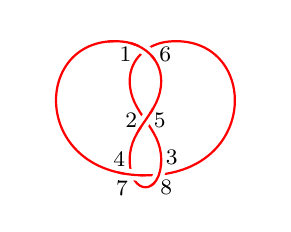
\begin{tikzpicture}
            \begin{knot}[
                clip width=5,
                clip radius=3pt,
                consider self intersections,
                ignore endpoint intersections=false
            ]
                \strand [red,thick] (-0.3,1)
                    to [out=-5,in=90] (0.2,0.5)
                    to [out=-90,in=90] (-0.2,-0.5)
                    to [out=-90,in=-90,looseness=3] (0.2,-0.5)
                    to [out=90,in=-90] (-0.2,0.5)
                    to [out=90,in=-175] (0.3,1)
                    to [out=5,in=0,out looseness=1.7,in looseness=2.2] (0,-0.7)
                    to [out=180,in=175,out looseness=2.2,in looseness=1.7] cycle
                ;
                \flipcrossings{3,5}
            \end{knot}
            \footnotesize
            \fill (0,0.89) circle (0pt)
                node[left,xshift=-2pt,yshift=-1.5pt]{1}
                node[right,xshift=2pt,yshift=-1.5pt]{6}
            ;
            \fill (0,0) circle (0pt)
                node[left]{2}
                node[right]{5}
            ;
            \fill (0.17,-0.69) circle (0pt)
                node[above right,xshift=-0.5pt,yshift=0.5pt]{3}
                node[below right,xshift=-2.5pt,yshift=1pt]{8}
            ;
            \fill (-0.17,-0.69) circle (0pt)
                node[above left,xshift=0.5pt]{4}
                node[below left,xshift=1.5pt,yshift=0.5pt]{7}
            ;
        \end{tikzpicture}
        \caption{Dowker labeling $a$.}
        \label{fig:fig8Dowkera}
    \end{subfigure}
    \begin{subfigure}[b]{0.3\linewidth}
        \centering
        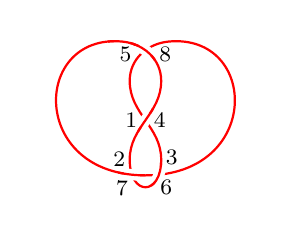
\begin{tikzpicture}
            \begin{knot}[
                clip width=5,
                clip radius=3pt,
                consider self intersections,
                ignore endpoint intersections=false
            ]
                \strand [red,thick] (-0.3,1)
                    to [out=-5,in=90] (0.2,0.5)
                    to [out=-90,in=90] (-0.2,-0.5)
                    to [out=-90,in=-90,looseness=3] (0.2,-0.5)
                    to [out=90,in=-90] (-0.2,0.5)
                    to [out=90,in=-175] (0.3,1)
                    to [out=5,in=0,out looseness=1.7,in looseness=2.2] (0,-0.7)
                    to [out=180,in=175,out looseness=2.2,in looseness=1.7] cycle
                ;
                \flipcrossings{3,5}
            \end{knot}
            \footnotesize
            \fill (0,0.89) circle (0pt)
                node[left,xshift=-2pt,yshift=-1.5pt]{5}
                node[right,xshift=2pt,yshift=-1.5pt]{8}
            ;
            \fill (0,0) circle (0pt)
                node[left]{1}
                node[right]{4}
            ;
            \fill (0.17,-0.69) circle (0pt)
                node[above right,xshift=-0.5pt,yshift=0.5pt]{3}
                node[below right,xshift=-2.5pt,yshift=1pt]{6}
            ;
            \fill (-0.17,-0.69) circle (0pt)
                node[above left,xshift=0.5pt]{2}
                node[below left,xshift=1.5pt,yshift=0.5pt]{7}
            ;
        \end{tikzpicture}
        \caption{Dowker labeling $b$.}
        \label{fig:fig8Dowkerb}
    \end{subfigure}
    \caption{The figure-eight knot labeled in Dowker notation.}
    \label{fig:fig8Dowker}
\end{figure}

However, there are multiple ways to Dowker-label the figure-eight knot. Two such labelings$^[$\footnote{Note that the labelings are shown without their accompanying orientations. However, these orientations should be self-evident on account of the numbering.}$^]$ (with an important difference between them) are shown in Figure \ref{fig:fig8Dowker}.\par

\begin{table}[h!]
    \centering
    \begin{subtable}[b]{0.3\linewidth}
        \centering
        \begin{tabular}{cccc}
            6 & 5 & 8 & 7\\
            1 & 2 & 3 & 4
        \end{tabular}
        \caption{Reconstruction pairing $a$.}
        \label{tab:fig8Dowkera}
    \end{subtable}
    \begin{subtable}[b]{0.3\linewidth}
        \centering
        \begin{tabular}{cccc}
            4 & 7 & 6 & 8\\
            1 & 2 & 3 & 5
        \end{tabular}
        \caption{Reconstruction pairing $b$.}
        \label{tab:fig8Dowkerb}
    \end{subtable}
    \caption{Dowker pairs for the figure-eight knot.}
    \label{tab:fig8Dowker}
\end{table}

Sort the numbers into reconstruction pairings, as in Table \ref{tab:fig8Dowker}. From this ordering of the pairings, the important difference may begin to show: while the integers one through four are all in different pairs in Table \ref{tab:fig8Dowkera}, one and four are paired up in Table \ref{tab:fig8Dowkerb}. The implications of this finding will soon become apparent.\par

\begin{figure}[h!]
    \centering
    \begin{subfigure}[b]{0.4\linewidth}
        \centering
        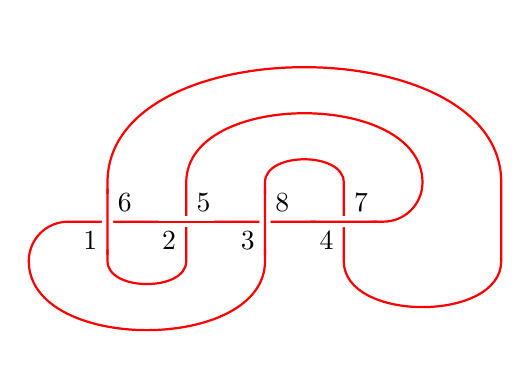
\begin{tikzpicture}[
            every node/.append style={black}
        ]
            \begin{knot}[
                clip width=5,
                consider self intersections
            ]
                \strand [red,thick] (0.5,0)
                    to (4.5,0)
                    to [out=0,in=-90] (5,0.5)
                    to [out=90,in=90] (2,0.5)
                    to node[below left]{2} node[above right]{5} (2,-0.5)
                    to [out=-90,in=-90] (1,-0.5)
                    to node[below left]{1} node[above right]{6} (1,0.5)
                    to [out=90,in=90] (6,0.5)
                    to (6,-0.5)
                    to [out=-90,in=-90] (4,-0.5)
                    to node[below left]{4} node[above right]{7} (4,0.5)
                    to [out=90,in=90] (3,0.5)
                    to node[below left]{3} node[above right]{8} (3,-0.5)
                    to [out=-90,in=-90] (0,-0.5)
                    to [out=90,in=180] cycle
                ;
                \flipcrossings{2,4}
            \end{knot}
        \end{tikzpicture}
        \caption{Reconstruction $a$.}
        \label{fig:fig8recona}
    \end{subfigure}
    \begin{subfigure}[b]{0.4\linewidth}
        \centering
        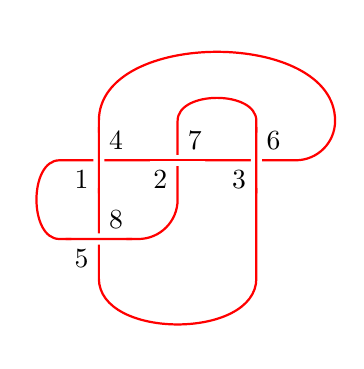
\begin{tikzpicture}[
            every node/.append style={black}
        ]
            \begin{knot}[
                clip width=5,
                consider self intersections
            ]
                \strand [red,thick] (0.5,0)
                    to (3.5,0)
                    to [out=0,in=-90] (4,0.5)
                    to [out=90,in=90] (1,0.5)
                    to node[below left]{1} node[above right]{4} (1,-0.5)
                    to node[below left]{5} node[above right]{8} (1,-1.5)
                    to [out=-90,in=-90] (3,-1.5)
                    to (3,-0.5)
                    to node[below left]{3} node[above right]{6} (3,0.5)
                    to [out=90,in=90] (2,0.5)
                    to node[below left]{2} node[above right]{7} (2,-0.5)
                    to [out=-90,in=0] (1.5,-1)
                    to (0.5,-1)
                    to [out=180,in=180] cycle
                ;
                \flipcrossings{1,2,4}
            \end{knot}
        \end{tikzpicture}
        \caption{Reconstruction $b$.}
        \label{fig:fig8reconb}
    \end{subfigure}
    \caption{Reconstructions of the figure-eight knot.}
    \label{fig:fig8recon}
\end{figure}

Reconstruct knot projections from the pairings in Table \ref{tab:fig8Dowker} to yield Figure \ref{fig:fig8recon}. This should make the difference more apparent.\par

\begin{figure}[h!]
    \centering
    \begin{subfigure}[b]{0.4\linewidth}
        \centering
        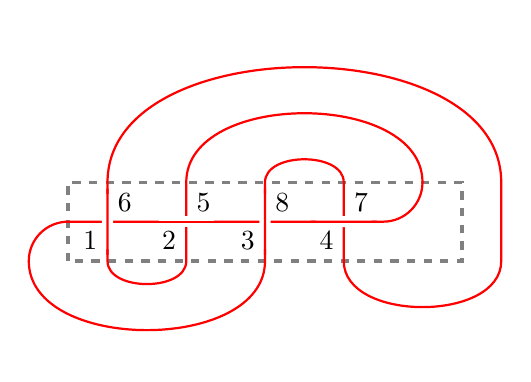
\begin{tikzpicture}[
            every node/.append style={black}
        ]
            \draw [gax,very thick,dashed] (0.5,-0.5) rectangle (5.5,0.5);
            \begin{knot}[
                clip width=5,
                consider self intersections
            ]
                \strand [red,thick] (0.5,0)
                    to (4.5,0)
                    to [out=0,in=-90] (5,0.5)
                    to [out=90,in=90] (2,0.5)
                    to node[below left]{2} node[above right]{5} (2,-0.5)
                    to [out=-90,in=-90] (1,-0.5)
                    to node[below left]{1} node[above right]{6} (1,0.5)
                    to [out=90,in=90] (6,0.5)
                    to (6,-0.5)
                    to [out=-90,in=-90] (4,-0.5)
                    to node[below left]{4} node[above right]{7} (4,0.5)
                    to [out=90,in=90] (3,0.5)
                    to node[below left]{3} node[above right]{8} (3,-0.5)
                    to [out=-90,in=-90] (0,-0.5)
                    to [out=90,in=180] cycle
                ;
                \flipcrossings{2,4}
            \end{knot}
        \end{tikzpicture}
        \caption{Reconstruction $a$.}
        \label{fig:fig8klzna}
    \end{subfigure}
    \begin{subfigure}[b]{0.4\linewidth}
        \centering
        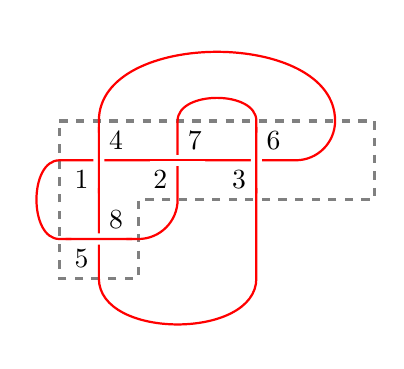
\begin{tikzpicture}[
            every node/.append style={black}
        ]
            \draw [gax,very thick,dashed] (0.5,0.5)
                -- (4.5,0.5)
                -- (4.5,-0.5)
                -- (1.5,-0.5)
                -- (1.5,-1.5)
                -- (0.5,-1.5)
                -- cycle
            ;
            \begin{knot}[
                clip width=5,
                consider self intersections
            ]
                \strand [red,thick] (0.5,0)
                    to (3.5,0)
                    to [out=0,in=-90] (4,0.5)
                    to [out=90,in=90] (1,0.5)
                    to node[below left]{1} node[above right]{4} (1,-0.5)
                    to node[below left]{5} node[above right]{8} (1,-1.5)
                    to [out=-90,in=-90] (3,-1.5)
                    to (3,-0.5)
                    to node[below left]{3} node[above right]{6} (3,0.5)
                    to [out=90,in=90] (2,0.5)
                    to node[below left]{2} node[above right]{7} (2,-0.5)
                    to [out=-90,in=0] (1.5,-1)
                    to (0.5,-1)
                    to [out=180,in=180] cycle
                ;
                \flipcrossings{1,2,4}
            \end{knot}
        \end{tikzpicture}
        \caption{Reconstruction $b$.}
        \label{fig:fig8klznb}
    \end{subfigure}
    \caption{The killzone in the figure-eight knot.}
    \label{fig:fig8klzn}
\end{figure}

Outlining the killzone in each, as in Figure \ref{fig:fig8klzn}, should make the difference fully apparent. While the killzone is rectangular in Figure \ref{fig:fig8klzna}, it is merely a rectilinear polygon in Figure \ref{fig:fig8klznb}. Because of the linearity of the killzone in Figure \ref{fig:fig8recona}, it is a superior starting projection for reducing bridge number.\par
There was a way to tell, even from the get-go, that the Dowker labeling in Figure \ref{fig:fig8Dowkerb} was not the best. In Figure \ref{fig:fig8Dowkera}, each crossing is passed through once before being passed through again while in Figure \ref{fig:fig8Dowkerb}, only three crossings are passed through before revisiting a previous crossing. This may be obvious, but it is critical to understand the following self-evident theorem.

\begin{theor}
    The number of crossings traversed before returning to a previously numbered crossing when labeling is equal to the number of crossings on the base strand in the Dowker reconstruction.
\end{theor}

As such, one should always try to maximize this number. Even if the issue escaped notice while labeling, the resultant pairings in Table \ref{tab:fig8Dowkerb} throw up an unmistakable numerical red flag --- \emph{whenever there is a skipped number in the bottom row, one should look for a superior Dowker labeling}.\par
At this point, two more definitions (below) will help clarify what constitutes the best possible Dowker labeling.

\begin{defi}
    \begin{description}
        \item[Superior killzone] \hfill \\ The killzone that maintains its rectangularity until the highest possible integer; the longest killzone that can be constructed (for a knot).
        \item[Ideal killzone] \hfill \\ A rectangular killzone.
    \end{description}
\end{defi}

Thus, the killzone in Figure \ref{fig:fig8klzna} is the superior killzone for the figure-eight knot (and, fortunately, is ideal) while the killzone in Figure \ref{fig:fig8klznb} is just a killzone.


\subsubsection{Reducing the Number of Bridges in the Figure-Eight Knot}\label{ss2:fig8reduce}
The "flip" employed between Figure \ref{fig:trefoilclra} and \ref{fig:trefoilclrb} is clearly a powerful tool for reducing bridge number. However, as this example will demonstrate, sometimes other moves are needed.\par

\begin{figure}[h!]
    \centering
    \begin{subfigure}[b]{0.4\linewidth}
        \centering
        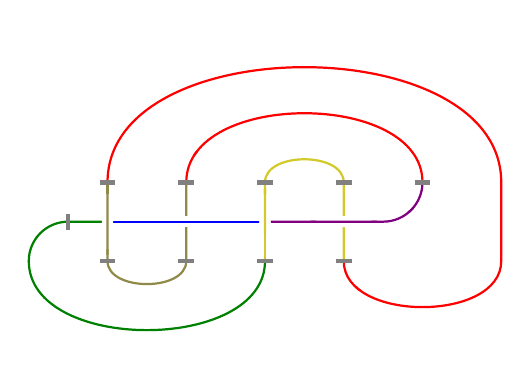
\begin{tikzpicture}
            \begin{knot}[
                clip width=5,
                consider self intersections,
                ignore endpoint intersections=false
            ]
                \strand [blue,thick] (1,0) to (3,0);
                \strand [pux,thick] (3,0)
                    to (4.5,0)
                    to [out=0,in=-90] (5,0.5)
                ;
                \strand [red,thick] (5,0.5) to [out=90,in=90] (2,0.5);
                \strand [yly,thick] (2,0.5)
                    to (2,-0.5)
                    to [out=-90,in=-90] (1,-0.5)
                    to (1,0.5)
                ;
                \strand [red,thick] (1,0.5)
                    to [out=90,in=90] (6,0.5)
                    to (6,-0.5)
                    to [out=-90,in=-90] (4,-0.5)
                ;
                \strand [ylz,thick] (4,-0.5)
                    to (4,0.5)
                    to [out=90,in=90] (3,0.5)
                    to (3,-0.5)
                ;
                \strand [grx,thick] (3,-0.5)
                    to [out=-90,in=-90] (0,-0.5)
                    to [out=90,in=180] (0.5,0)
                    to (1,0)
                ;
                \flipcrossings{3,5}
            \end{knot}
            \node [verti] at (0.5,0) {};
            \node [horiz] at (5,0.5) {};
            \foreach \x in {1,2,3,4} {
                \foreach \y in {-0.5,0.5} {
                    \node [horiz] at (\x,\y) {};
                }
            }
        \end{tikzpicture}
        \caption{4 bridges.}
        \label{fig:fig8clra}
    \end{subfigure}
    \begin{subfigure}[b]{0.4\linewidth}
        \centering
        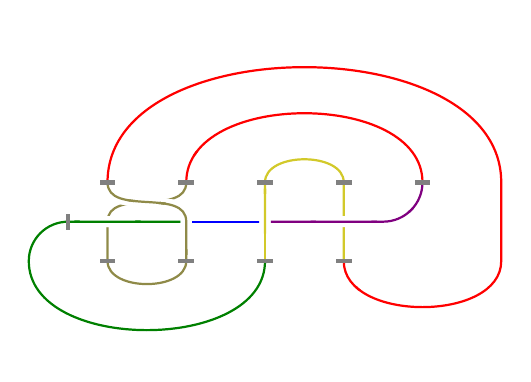
\begin{tikzpicture}
            \begin{knot}[
                clip width=5,
                consider self intersections,
                ignore endpoint intersections=false
            ]
                \strand [blue,thick] (2,0) to (3,0);
                \strand [pux,thick] (3,0)
                    to (4.5,0)
                    to [out=0,in=-90] (5,0.5)
                ;
                \strand [red,thick] (5,0.5) to [out=90,in=90] (2,0.5);
                \strand [yly,thick] (2,0.5)
                    to [out=-90,in=90] (1,0)
                    to (1,-0.5)
                    to [out=-90,in=-90] (2,-0.5)
                    to (2,0)
                    to [out=90,in=-90] (1,0.5)
                ;
                \strand [red,thick] (1,0.5)
                    to [out=90,in=90] (6,0.5)
                    to (6,-0.5)
                    to [out=-90,in=-90] (4,-0.5)
                ;
                \strand [ylz,thick] (4,-0.5)
                    to (4,0.5)
                    to [out=90,in=90] (3,0.5)
                    to (3,-0.5)
                ;
                \strand [grx,thick] (3,-0.5)
                    to [out=-90,in=-90] (0,-0.5)
                    to [out=90,in=180] (0.5,0)
                    to (2,0)
                ;
                \flipcrossings{3,5,8,9,10}
            \end{knot}
            \node [verti] at (0.5,0) {};
            \node [horiz] at (5,0.5) {};
            \foreach \x in {1,2,3,4} {
                \foreach \y in {-0.5,0.5} {
                    \node [horiz] at (\x,\y) {};
                }
            }
        \end{tikzpicture}
        \caption{3 bridges (left).}
        \label{fig:fig8clrb}
    \end{subfigure}
    \begin{subfigure}[b]{0.4\linewidth}
        \centering
        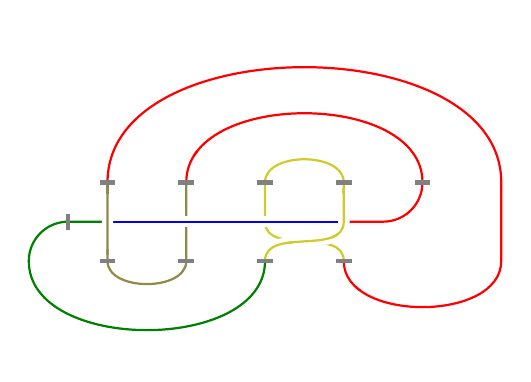
\begin{tikzpicture}
            \begin{knot}[
                clip width=5,
                consider self intersections,
                ignore endpoint intersections=false
            ]
                \strand [blue,thick] (1,0) to (4,0);
                \strand [red,thick] (4,0)
                    to (4.5,0)
                    to [out=0,in=-90] (5,0.5)
                    to [out=90,in=90] (2,0.5);
                \strand [yly,thick] (2,0.5)
                    to (2,-0.5)
                    to [out=-90,in=-90] (1,-0.5)
                    to (1,0.5)
                ;
                \strand [red,thick] (1,0.5)
                    to [out=90,in=90] (6,0.5)
                    to (6,-0.5)
                    to [out=-90,in=-90] (4,-0.5)
                ;
                \strand [ylz,thick] (4,-0.5)
                    to [out=90,in=-90] (3,0)
                    to (3,0.5)
                    to [out=90,in=90] (4,0.5)
                    to (4,0)
                    to [out=-90,in=90] (3,-0.5)
                ;
                \strand [grx,thick] (3,-0.5)
                    to [out=-90,in=-90] (0,-0.5)
                    to [out=90,in=180] (0.5,0)
                    to (1,0)
                ;
                \flipcrossings{6,7,8,13}
            \end{knot}
            \node [verti] at (0.5,0) {};
            \node [horiz] at (5,0.5) {};
            \foreach \x in {1,2,3,4} {
                \foreach \y in {-0.5,0.5} {
                    \node [horiz] at (\x,\y) {};
                }
            }
        \end{tikzpicture}
        \caption{3 bridges (right).}
        \label{fig:fig8clrc}
    \end{subfigure}
    \begin{subfigure}[b]{0.4\linewidth}
        \centering
        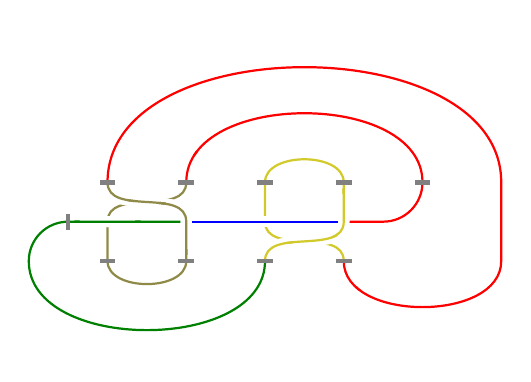
\begin{tikzpicture}
            \begin{knot}[
                clip width=5,
                consider self intersections,
                ignore endpoint intersections=false
            ]
                \strand [blue,thick] (2,0) to (4,0);
                \strand [red,thick] (4,0)
                    to (4.5,0)
                    to [out=0,in=-90] (5,0.5)
                    to [out=90,in=90] (2,0.5);
                \strand [yly,thick] (2,0.5)
                    to [out=-90,in=90] (1,0)
                    to (1,-0.5)
                    to [out=-90,in=-90] (2,-0.5)
                    to (2,0)
                    to [out=90,in=-90] (1,0.5)
                ;
                \strand [red,thick] (1,0.5)
                    to [out=90,in=90] (6,0.5)
                    to (6,-0.5)
                    to [out=-90,in=-90] (4,-0.5)
                ;
                \strand [ylz,thick] (4,-0.5)
                    to [out=90,in=-90] (3,0)
                    to (3,0.5)
                    to [out=90,in=90] (4,0.5)
                    to (4,0)
                    to [out=-90,in=90] (3,-0.5)
                ;
                \strand [grx,thick] (3,-0.5)
                    to [out=-90,in=-90] (0,-0.5)
                    to [out=90,in=180] (0.5,0)
                    to (2,0)
                ;
                \flipcrossings{6,7,8,10,11,12,17}
            \end{knot}
            \node [verti] at (0.5,0) {};
            \node [horiz] at (5,0.5) {};
            \foreach \x in {1,2,3,4} {
                \foreach \y in {-0.5,0.5} {
                    \node [horiz] at (\x,\y) {};
                }
            }
        \end{tikzpicture}
        \caption{3 bridges (both).}
        \label{fig:fig8clrd}
    \end{subfigure}
    \caption{Combining and shifting bridges in the figure-eight knot.}
    \label{fig:fig8clr}
\end{figure}

In Figure \ref{fig:fig8clra}, there are two loops (\textcolor{yly}{dark yellow} and \textcolor{ylz}{light yellow}) around the killzone similar to the \textcolor{ylx}{yellow} loop in Figure \ref{fig:trefoilclra}. Making the same move as between Figure \ref{fig:trefoilclra} and \ref{fig:trefoilclrb} on either strand will reduce the number of bridges by one. However, making the move on both will still only reduce the number of bridges by one. This occurs because the first of the two moves combines two bridges while the second only shifts a bridge. The combining/shifting is reflected in the projections of Figure \ref{fig:fig8clr}. From Figure \ref{fig:fig8clra} to \ref{fig:fig8clrb}, the \textcolor{grx}{green}/\textcolor{ylz}{light yellow} and \textcolor{blue}{blue} bridges are combined$^[$\footnote{Note that a \textcolor{blue}{blue} understrand remains in Figure \ref{fig:fig8clrb} to make the transition from Figure \ref{fig:fig8clrb} to \ref{fig:fig8clrd} more easily parsed.}$^]$. From Figure \ref{fig:fig8clra} to \ref{fig:fig8clrc}, the \textcolor{blue}{blue} and \textcolor{pux}{purple} bridges are combined. However, from Figure \ref{fig:fig8clrb} to \ref{fig:fig8clrd}, the \textcolor{pux}{purple} bridge gives way to a \textcolor{blue}{blue} bridge and from Figure \ref{fig:fig8clrc} to \ref{fig:fig8clrd}, the \textcolor{blue}{blue} bridge shrinks and the \textcolor{grx}{green}/\textcolor{ylz}{light yellow} bridge expands.\par
In light of the failure of the second move to further reduce the number of bridges, the move may seem extraneous; it may seem that proceeding from Figure \ref{fig:fig8clrb} or \ref{fig:fig8clrc} would be cleaner. However, because Figure \ref{fig:fig8clrd} contains a one-crossing bridge entirely within the bounds of the killzone, one should continue reducing the number of bridges from it.\par
Let's justify the previous assertion in two parts as follows.

\begin{conj}
    \begin{enumerate}
        \item It is preferable to work with a one-crossing bridge.
        \item It is preferable to work with a bridge existing entirely within the killzone.
    \end{enumerate}
\end{conj}

Notably, every bridge removed thus far (one in Figure \ref{fig:trefoilclr} and one in Figure \ref{fig:fig8clr}) has been a one-crossing bridge (literally a bridge that spans only one crossing). Logically, because there is only one crossing beneath a one-crossing bridge, a cleaner projection results from shifting that crossing. Likewise, every bridge removed thus far has been contained entirely within the killzone. By the definition of the killzone, all strands are in a small, organized region, thereby clarifying the relationship between a knot's key elements.

\begin{figure}[h!]
    \centering
    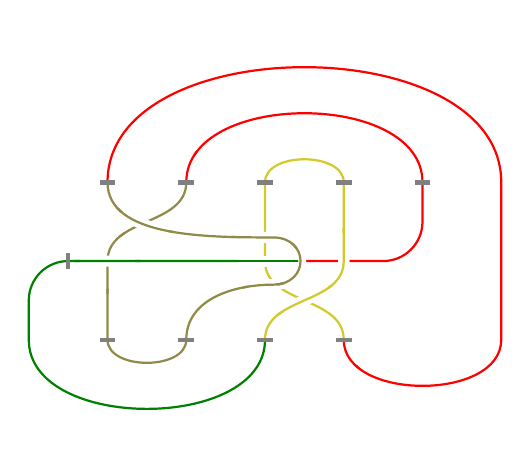
\begin{tikzpicture}
        \begin{knot}[
            clip width=5,
            consider self intersections,
            ignore endpoint intersections=false
        ]
            \strand [red,thick] (3.5,0)
                to (4.5,0)
                to [out=0,in=-90] (5,0.5)
                to (5,1)
                to [out=90,in=90] (2,1);
            \strand [yly,thick] (2,1)
                to [out=-90,in=90] (1,0)
                to (1,-1)
                to [out=-90,in=-90] (2,-1)
                to [out=90,in=180] (3.1,-0.3)
                to [out=0,in=0,looseness=2] (3.1,0.3)
                to [out=180,in=-90,in looseness=0.8] (1,1)
            ;
            \strand [red,thick] (1,1)
                to [out=90,in=90] (6,1)
                to (6,-1)
                to [out=-90,in=-90] (4,-1)
            ;
            \strand [ylz,thick] (4,-1)
                to [out=90,in=-90] (3,0)
                to (3,1)
                to [out=90,in=90] (4,1)
                to (4,0)
                to [out=-90,in=90] (3,-1)
            ;
            \strand [grx,thick] (3,-1)
                to [out=-90,in=-90] (0,-1)
                to (0,-0.5)
                to [out=90,in=180] (0.5,0)
                to (3.5,0)
            ;
            \flipcrossings{1,2,4,6,13,14,15}
        \end{knot}
        \node [verti] at (0.5,0) {};
        \node [horiz] at (5,1) {};
        \foreach \x in {1,2,3,4} {
            \foreach \y in {-1,1} {
                \node [horiz] at (\x,\y) {};
            }
        }
    \end{tikzpicture}
    \caption{A new move in the figure-eight knot.}
    \label{fig:fig8clr-2}
\end{figure}

Proceeding with Figure \ref{fig:fig8clrd}, it should be clear that the move that has been used thus far cannot be used again (there are no more loops around the killzone that have not already been "flipped"). Therefore, a new move is needed. If we freeze the strands outside the killzone, as intended, imagine that the segments within can "wiggle around" a bit, distorting themselves at will via planar isotropies and moored only at either end by the dashes (killzone boundaries). In the course of their wiggling, one strand might pass over another crossing --- this is key. If the \textcolor{yly}{dark yellow} strand can "wiggle" past and over the top of the crossing to the right, as in Figure \ref{fig:fig8clr-2}, \emph{there will no longer be an understrand (part of the \textcolor{ylz}{light yellow} bridge) separating the \textcolor{grx}{green} bridge and the \textcolor{red}{red} strand past the \textcolor{blue}{blue} bridge} and \emph{no new bridges will have been created}.\par

\begin{figure}[h!]
    \centering
    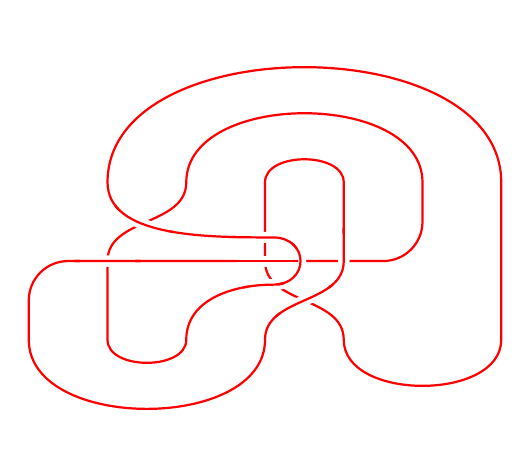
\begin{tikzpicture}
        \begin{knot}[
            clip width=5,
            consider self intersections,
            ignore endpoint intersections=false
        ]
            \strand [red,thick] (3.5,0)
                to (4.5,0)
                to [out=0,in=-90] (5,0.5)
                to (5,1)
                to [out=90,in=90] (2,1)
                to [out=-90,in=90] (1,0)
                to (1,-1)
                to [out=-90,in=-90] (2,-1)
                to [out=90,in=180] (3.1,-0.3)
                to [out=0,in=0,looseness=2] (3.1,0.3)
                to [out=180,in=-90,in looseness=0.8] (1,1)
                to [out=90,in=90] (6,1)
                to (6,-1)
                to [out=-90,in=-90] (4,-1)
                to [out=90,in=-90] (3,0)
                to (3,1)
                to [out=90,in=90] (4,1)
                to (4,0)
                to [out=-90,in=90] (3,-1)
                to [out=-90,in=-90] (0,-1)
                to (0,-0.5)
                to [out=90,in=180] (0.5,0)
                to cycle
            ;
            \flipcrossings{1,2,3,4,5,10,11,12}
        \end{knot}
    \end{tikzpicture}
    \caption{A projection of the figure-eight knot with 2 bridges.}
    \label{fig:fig8fin}
\end{figure}

Because $b(4_1)=2$, Figure \ref{fig:fig8clr-2} is a minimal-bridge projection. This projection is cleaned up in Figure \ref{fig:fig8fin}.


\subsubsection{Reducing the Number of Bridges in the Trefoil Knot with the New Move}\label{ss2:trefoilreduce-2}
Note that the new move (the move introduced between Figure \ref{fig:fig8clrd} and \ref{fig:fig8clr-2}) is, in fact, not new. Rather, it made an earlier appearance between the two subfigures of Figure \ref{fig:2altern}. In addition, the region circled in \textcolor{cyan}{cyan} in Figure \ref{fig:2altern} has been seen since --- it is the complete killzone of the trefoil knot (see Figure \ref{fig:trefoilklzna}) and the left part of the killzone of the figure-eight knot (see Figure \ref{fig:fig8klzna}). Thus, by the proof associated with Figure \ref{fig:2altern} and experience with the figure-eight knot, the move in Figure \ref{fig:2altern} should be able to remove the one removable bridge in the trefoil knot and at least one of the removable bridges in the figure-eight knot. Let's see if this holds true.\par

\begin{figure}[h!]
    \centering
    \begin{subfigure}[b]{0.35\linewidth}
        \centering
        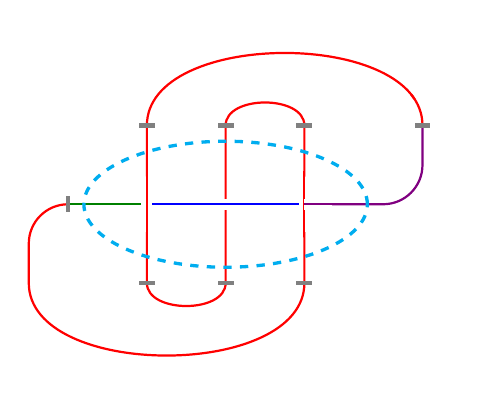
\begin{tikzpicture}
            \begin{knot}[
                clip width=5,
                consider self intersections,
                ignore endpoint intersections=false
            ]
                \strand [grx,thick] (0,0) to (1,0);
                \strand [blue,thick] (1,0) to (3,0);
                \strand [pux,thick] (3,0)
                    to (4,0)
                    to [out=0,in=-90] (4.5,0.5)
                    to (4.5,1)
                ;
                \strand [red,thick] (4.5,1)
                    to [out=90,in=90,looseness=0.9] (1,1)
                    to (1,-1)
                    to [out=-90,in=-90] (2,-1)
                    to (2,1)
                    to [out=90,in=90] (3,1)
                    to (3,-1)
                    to [out=-90,in=-90,looseness=0.9] (-0.5,-1)
                    to (-0.5,-0.5)
                    to [out=90,in=180] (0,0)
                ;
                \flipcrossings{1,3,5,7}
            \end{knot}
            \node [verti] at (0,0) {};
            \node [horiz] at (4.5,1) {};
            \foreach \x in {1,2,3} {
                \foreach \y in {-1,1} {
                    \node [horiz] at (\x,\y) {};
                }
            }
            \draw[cyan,very thick,dashed] (2,0) ellipse (1.8cm and 0.8cm);
        \end{tikzpicture}
        \caption{3 bridges.}
        \label{fig:trefoilcirclea}
    \end{subfigure}
    \begin{subfigure}[b]{0.35\linewidth}
        \centering
        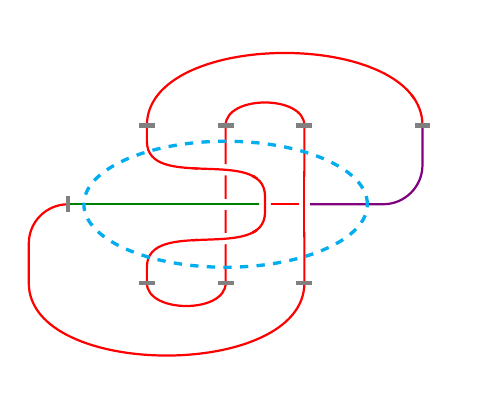
\begin{tikzpicture}
            \begin{knot}[
                clip width=5,
                consider self intersections,
                ignore endpoint intersections=false
            ]
                \strand [grx,thick] (0,0) to (2.5,0);
                \strand [red,thick] (2.5,0) to (3,0);
                \strand [pux,thick] (3,0)
                    to (4,0)
                    to [out=0,in=-90] (4.5,0.5)
                    to (4.5,1)
                ;
                \strand [red,thick] (4.5,1)
                    to [out=90,in=90,looseness=0.9] (1,1)
                    to (1,0.8)
                    to [out=-90,in=90] (2.5,0.1)
                    to (2.5,-0.1)
                    to [out=-90,in=90] (1,-0.8)
                    to (1,-1)
                    to [out=-90,in=-90] (2,-1)
                    to (2,1)
                    to [out=90,in=90] (3,1)
                    to (3,-1)
                    to [out=-90,in=-90,looseness=0.9] (-0.5,-1)
                    to (-0.5,-0.5)
                    to [out=90,in=180] (0,0)
                ;
                \flipcrossings{1,4,6,7}
            \end{knot}
            \node [verti] at (0,0) {};
            \node [horiz] at (4.5,1) {};
            \foreach \x in {1,2,3} {
                \foreach \y in {-1,1} {
                    \node [horiz] at (\x,\y) {};
                }
            }
            \draw[cyan,very thick,dashed] (2,0) ellipse (1.8cm and 0.8cm);
        \end{tikzpicture}
        \caption{2 bridges.}
        \label{fig:trefoilcircleb}
    \end{subfigure}
    \caption{Combining bridges with the new move in the trefoil knot.}
    \label{fig:trefoilcircle}
\end{figure}

Take the projection of the trefoil knot in Figure \ref{fig:trefoilklznb} and circle the region in \textcolor{cyan}{cyan}, as in Figure \ref{fig:trefoilcirclea}, that corresponds to the encircled region of Figure \ref{fig:2alterna}. Perform the new move to generate Figure \ref{fig:trefoilcircleb} and notice that one bridge is removed. Therefore, Figure \ref{fig:trefoilcircleb} is another minimal-bridge projection of the trefoil knot.\par
Although it will not be shown here, the same thing would indeed work with the figure-eight knot, as alluded to above. However, unlike the trefoil knot, there are two opportunities to employ the new move within the killzone of the figure-eight knot. Unfortunately, for the same reason that two renditions of the first move did not remove two bridges in Figure \ref{fig:fig8clr}, two renditions of the new move would also only remove one bridge.


\subsection{Bridging Moves}\label{sss:bridging}
Section \ref{sss:evidence} introduced three techniques for finding projections with the minimal number of bridges. This section will more rigorously define those strategies and explore their properties.\par
The first technique introduced was the aptly named killzone. This procedure will not be discussed at length here since it and two of its derivatives (the superior and ideal killzone) have already been given formal definitions. Suffice to say generating the killzone is perfectly legal because a Dowker reconstruction and the original projection can be interconverted via a planar isotropy.\par
The two moves used to actually remove bridges will be explored at length. Since their definitions are based in the Reidemeister moves, those will presently be defined.\par

\begin{figure}[h!]
    \centering
    \begin{subfigure}[b]{0.6\linewidth}
        \centering
        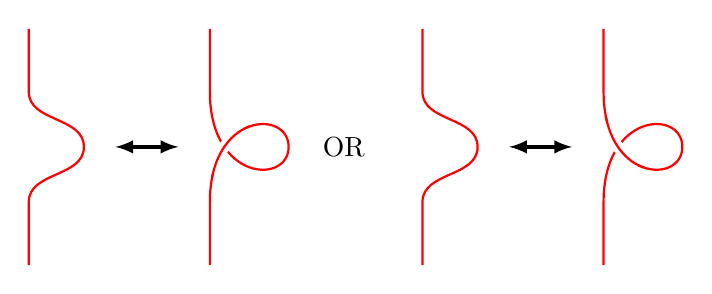
\begin{tikzpicture}
            \begin{scope}[
                xshift=-2.5cm
            ]
                \draw[very thick,latex-latex] (-0.4,0) -- (0.4,0);
                \begin{scope}[
                    xshift=-1.5cm
                ]
                    \draw [red,thick] (0,-1.5)
                        to (0,-0.7)
                        to [out=90,in=-90] (0.7,0)
                        to [out=90,in=-90] (0,0.7)
                        to (0,1.5)
                    ;
                \end{scope}
                \begin{knot}[
                    xshift=0.8cm,
                    clip width=5,
                    consider self intersections=no splits
                ]
                    \strand [red,thick] (0,-1.5)
                        to (0,-0.7)
                        to [out=90,in=90,out looseness=2.4] (1,0)
                        to [out=-90,in=-90,in looseness=2.4] (0,0.7)
                        to (0,1.5)
                    ;
                \end{knot}
            \end{scope}
            \node{OR};
            \begin{scope}[
                xshift=2.5cm
            ]
                \draw[very thick,latex-latex] (-0.4,0) -- (0.4,0);
                \begin{scope}[
                    xshift=-1.5cm
                ]
                    \draw [red,thick] (0,-1.5)
                        to (0,-0.7)
                        to [out=90,in=-90] (0.7,0)
                        to [out=90,in=-90] (0,0.7)
                        to (0,1.5)
                    ;
                \end{scope}
                \begin{knot}[
                    xshift=0.8cm,
                    clip width=5,
                    consider self intersections=no splits
                ]
                    \strand [red,thick] (0,-1.5)
                        to (0,-0.7)
                        to [out=90,in=90,out looseness=2.4] (1,0)
                        to [out=-90,in=-90,in looseness=2.4] (0,0.7)
                        to (0,1.5)
                    ;
                    \flipcrossings{1}
                \end{knot}
            \end{scope}
        \end{tikzpicture}
        \caption{Type I Reidemeister moves.}
        \label{fig:reidema}
    \end{subfigure}\\
    \vspace{1em}
    \begin{subfigure}[b]{0.6\linewidth}
        \centering
        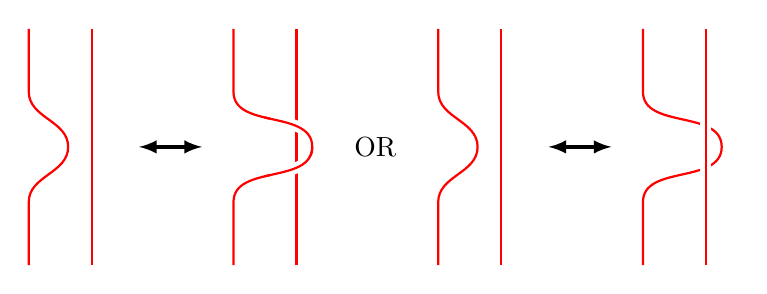
\begin{tikzpicture}
            \begin{scope}[
                xshift=-2.6cm
            ]
                \draw[very thick,latex-latex] (-0.4,0) -- (0.4,0);
                \begin{scope}[
                    xshift=-1.8cm
                ]
                    \draw [red,thick] (0,-1.5)
                        to (0,-0.7)
                        to [out=90,in=-90] (0.5,0)
                        to [out=90,in=-90] (0,0.7)
                        to (0,1.5)
                    ;
                    \draw [red,thick] (0.8,-1.5) -- (0.8,1.5);
                \end{scope}
                \begin{knot}[
                    xshift=0.8cm,
                    clip width=5
                ]
                    \strand [red,thick] (0,-1.5)
                        to (0,-0.7)
                        to [out=90,in=-90] (1,0)
                        to [out=90,in=-90] (0,0.7)
                        to (0,1.5)
                    ;
                    \strand [red,thick] (0.8,-1.5) to (0.8,1.5);
                \end{knot}
            \end{scope}
            \node{OR};
            \begin{scope}[
                xshift=2.6cm
            ]
                \draw[very thick,latex-latex] (-0.4,0) -- (0.4,0);
                \begin{scope}[
                    xshift=-1.8cm
                ]
                    \draw [red,thick] (0,-1.5)
                        to (0,-0.7)
                        to [out=90,in=-90] (0.5,0)
                        to [out=90,in=-90] (0,0.7)
                        to (0,1.5)
                    ;
                    \draw [red,thick] (0.8,-1.5) -- (0.8,1.5);
                \end{scope}
                \begin{knot}[
                    xshift=0.8cm,
                    clip width=5
                ]
                    \strand [red,thick] (0,-1.5)
                        to (0,-0.7)
                        to [out=90,in=-90] (1,0)
                        to [out=90,in=-90] (0,0.7)
                        to (0,1.5)
                    ;
                    \strand [red,thick] (0.8,-1.5) to (0.8,1.5);
                    \flipcrossings{1,2}
                \end{knot}
            \end{scope}
        \end{tikzpicture}
        \caption{Type II Reidemeister moves.}
        \label{fig:reidemb}
    \end{subfigure}\\
    \vspace{1em}
    \begin{subfigure}[b]{\linewidth}
        \centering
        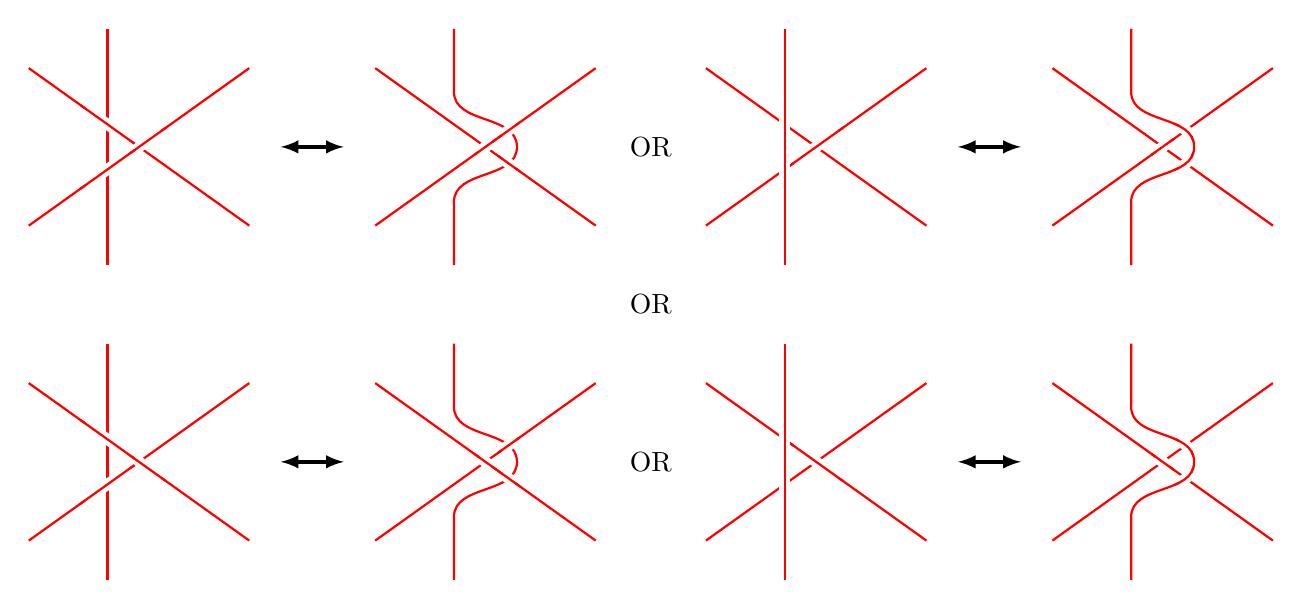
\begin{tikzpicture}
            \begin{scope}
                \begin{scope}[
                    xshift=-4.3cm
                ]
                    \draw[very thick,latex-latex] (-0.4,0) -- (0.4,0);
                    \begin{knot}[
                        xshift=-2.2cm,
                        every strand/.append style={red,thick},
                        clip width=5
                    ]
                        \strand (-1.4,-1) to (1.4,1);
                        \strand (-1.4,1) to (1.4,-1);
                        \strand (-0.4,-1.5) to (-0.4,1.5);
                    \end{knot}
                    \begin{knot}[
                        xshift=2.2cm,
                        every strand/.append style={red,thick},
                        clip width=5,
                        clip radius=3pt
                    ]
                        \strand (-1.4,-1) to (1.4,1);
                        \strand (-1.4,1) to (1.4,-1);
                        \strand [red,thick] (-0.4,-1.5)
                            to (-0.4,-0.7)
                            to [out=90,in=-90] (0.4,0)
                            to [out=90,in=-90] (-0.4,0.7)
                            to (-0.4,1.5)
                        ;
                    \end{knot}
                \end{scope}
                \node{OR};
                \begin{scope}[
                    xshift=4.3cm
                ]
                    \draw[very thick,latex-latex] (-0.4,0) -- (0.4,0);
                    \begin{knot}[
                        xshift=-2.2cm,
                        every strand/.append style={red,thick},
                        clip width=5
                    ]
                        \strand (-1.4,-1) to (1.4,1);
                        \strand (-1.4,1) to (1.4,-1);
                        \strand (-0.4,-1.5) to (-0.4,1.5);
                        \flipcrossings{2,3}
                    \end{knot}
                    \begin{knot}[
                        xshift=2.2cm,
                        every strand/.append style={red,thick},
                        clip width=5,
                        clip radius=3pt
                    ]
                        \strand (-1.4,-1) to (1.4,1);
                        \strand (-1.4,1) to (1.4,-1);
                        \strand [red,thick] (-0.4,-1.5)
                            to (-0.4,-0.7)
                            to [out=90,in=-90] (0.4,0)
                            to [out=90,in=-90] (-0.4,0.7)
                            to (-0.4,1.5)
                        ;
                        \flipcrossings{2,3}
                    \end{knot}
                \end{scope}
                \node at (0,-2) {OR};
                \begin{scope}[
                    yshift=-4cm
                ]
                    \begin{scope}[
                        xshift=-4.3cm
                    ]
                        \draw[very thick,latex-latex] (-0.4,0) -- (0.4,0);
                        \begin{knot}[
                            xshift=-2.2cm,
                            every strand/.append style={red,thick},
                            clip width=5
                        ]
                            \strand (-1.4,-1) to (1.4,1);
                            \strand (-1.4,1) to (1.4,-1);
                            \strand (-0.4,-1.5) to (-0.4,1.5);
                            \flipcrossings{1}
                        \end{knot}
                        \begin{knot}[
                            xshift=2.2cm,
                            every strand/.append style={red,thick},
                            clip width=5,
                            clip radius=3pt
                        ]
                            \strand (-1.4,-1) to (1.4,1);
                            \strand (-1.4,1) to (1.4,-1);
                            \strand [red,thick] (-0.4,-1.5)
                                to (-0.4,-0.7)
                                to [out=90,in=-90] (0.4,0)
                                to [out=90,in=-90] (-0.4,0.7)
                                to (-0.4,1.5)
                            ;
                            \flipcrossings{1}
                        \end{knot}
                    \end{scope}
                    \node{OR};
                    \begin{scope}[
                        xshift=4.3cm
                    ]
                        \draw[very thick,latex-latex] (-0.4,0) -- (0.4,0);
                        \begin{knot}[
                            xshift=-2.2cm,
                            every strand/.append style={red,thick},
                            clip width=5
                        ]
                            \strand (-1.4,-1) to (1.4,1);
                            \strand (-1.4,1) to (1.4,-1);
                            \strand (-0.4,-1.5) to (-0.4,1.5);
                            \flipcrossings{1,2,3}
                        \end{knot}
                        \begin{knot}[
                            xshift=2.2cm,
                            every strand/.append style={red,thick},
                            clip width=5,
                            clip radius=3pt
                        ]
                            \strand (-1.4,-1) to (1.4,1);
                            \strand (-1.4,1) to (1.4,-1);
                            \strand [red,thick] (-0.4,-1.5)
                                to (-0.4,-0.7)
                                to [out=90,in=-90] (0.4,0)
                                to [out=90,in=-90] (-0.4,0.7)
                                to (-0.4,1.5)
                            ;
                            \flipcrossings{1,2,3}
                        \end{knot}
                    \end{scope}
                \end{scope}
            \end{scope}
        \end{tikzpicture}
        \caption{Type III Reidemeister moves.}
        \label{fig:reidemc}
    \end{subfigure}
    \caption{The Reidemeister moves.}
    \label{fig:reidem}
\end{figure}
\newpage

\begin{defi}
    \begin{description}
        \item[Type I Reidemeister move] \hfill \\ \dq{Put in or take out a twist in the knot}{bib:knotbook}{13}
        \item[Type II Reidemeister move] \hfill \\ \dq{Either add two crossings or remove two crossings}{bib:knotbook}{13}
        \item[Type III Reidemeister move] \hfill \\ \dq{Slide a strand of the knot from one side of a crossing to the other side of the crossing}{bib:knotbook}{13}
    \end{description}
\end{defi}

In 1926, Kurt Reidemeister proved that two projections of the same knot can be interconverted using only the Reidemeister moves (see Figure \ref{fig:reidem}) and planar isotropies. Furthermore, Reidemeister moves are legal (transformations that do not change a projection of one knot into that of a different, distinct knot). Therefore, if the two moves used to remove bridges above are legal moves, there should be a sequence of Reidemeister moves that sums to them. First, however, define these "bridging moves" as follows.\par

\begin{figure}[h!]
    \centering
    \begin{subfigure}[b]{0.8\linewidth}
        \centering
        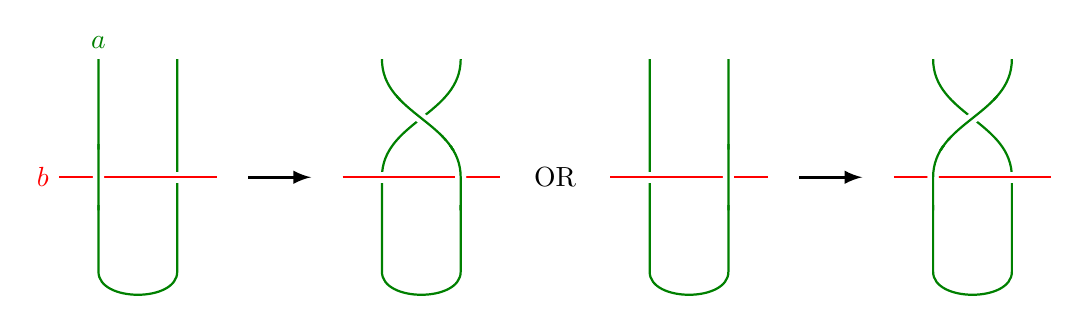
\begin{tikzpicture}
            \begin{scope}[
                xshift=-3.5cm
            ]
                \draw[very thick,-latex] (-0.4,0) -- (0.4,0);
                \begin{knot}[
                    xshift=-1.8cm,
                    clip width=5
                ]
                    \strand [grx,thick] (-0.5,1.5) node[above,grx]{$a$}
                        to (-0.5,-1.2)
                        to [out=-90,in=-90] (0.5,-1.2)
                        to (0.5,1.5)
                    ;
                    \strand [red,thick] (-1,0) node[left,red]{$b$} to (1,0);
                    \flipcrossings{2}
                \end{knot}
                \begin{knot}[
                    xshift=1.8cm,
                    clip width=5,
                    consider self intersections,
                    ignore endpoint intersections=false
                ]
                    \strand [grx,thick] (-0.5,1.5)
                        to [out=-90,in=90] (0.5,0)
                        to (0.5,-1.2)
                        to [out=-90,in=-90] (-0.5,-1.2)
                        to (-0.5,0)
                        to [out=90,in=-90] (0.5,1.5)
                    ;
                    \strand [red,thick] (-1,0) to (1,0);
                    \flipcrossings{4,5}
                \end{knot}
            \end{scope}
            \node{OR};
            \begin{scope}[
                xshift=3.5cm
            ]
                \draw[very thick,-latex] (-0.4,0) -- (0.4,0);
                \begin{knot}[
                    xshift=-1.8cm,
                    clip width=5
                ]
                    \strand [grx,thick] (-0.5,1.5)
                        to (-0.5,-1.2)
                        to [out=-90,in=-90] (0.5,-1.2)
                        to (0.5,1.5)
                    ;
                    \strand [red,thick] (-1,0) to (1,0);
                    \flipcrossings{1}
                \end{knot}
                \begin{knot}[
                    xshift=1.8cm,
                    clip width=5,
                    consider self intersections,
                    ignore endpoint intersections=false
                ]
                    \strand [grx,thick] (-0.5,1.5)
                        to [out=-90,in=90] (0.5,0)
                        to (0.5,-1.2)
                        to [out=-90,in=-90] (-0.5,-1.2)
                        to (-0.5,0)
                        to [out=90,in=-90] (0.5,1.5)
                    ;
                    \strand [red,thick] (-1,0) to (1,0);
                    \flipcrossings{1,2,3}
                \end{knot}
            \end{scope}
        \end{tikzpicture}
        \caption{Type I bridging moves.}
        \label{fig:bridgea}
    \end{subfigure}\\
    \vspace{1em}
    \begin{subfigure}[b]{0.6\linewidth}
        \centering
        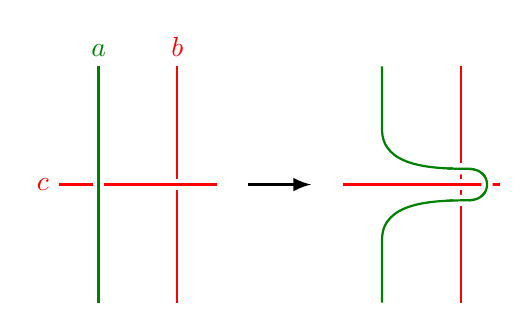
\begin{tikzpicture}
            \draw[very thick,-latex] (-0.4,0) -- (0.4,0);
            \begin{knot}[
                xshift=-1.8cm,
                clip width=5
            ]
                \strand [grx,thick] (-0.5,-1.5) to (-0.5,1.5) node[above,grx]{$a$};
                \strand [red,thick] (0.5,-1.5) to (0.5,1.5) node[above,red]{$b$};
                \strand [red,thick] (-1,0) node[left,red]{$c$} to (1,0);
                \flipcrossings{2}
            \end{knot}
            \begin{knot}[
                xshift=1.8cm,
                clip width=5,
                clip radius=3pt,
                ignore endpoint intersections=false
            ]
                \strand [grx,thick] (-0.5,-1.5)
                    to (-0.5,-0.7)
                    to [out=90,in=180] (0.6,-0.2)
                    to [out=0,in=0,looseness=2] (0.6,0.2)
                    to [out=180,in=-90] (-0.5,0.7)
                    to (-0.5,1.5)
                ;
                \strand [red,thick] (0.5,-1.5) to (0.5,1.5);
                \strand [red,thick] (-1,0) to (1,0);
                \flipcrossings{4}
            \end{knot}
        \end{tikzpicture}
        \caption{Type II bridging move.}
        \label{fig:bridgeb}
    \end{subfigure}
    \caption{The bridging moves.}
    \label{fig:bridge}
\end{figure}

\begin{defi}
    \begin{description}
        \item[Type I bridging move] \hfill \\ Given strand $a$ that passes over strand $b$ and then immediately passes under $b$ adjacent to the first crossing, flip $a$ over $b$ without shifting its endpoints such that a new crossing is created and the original two crossings are inverted.
        \item[Type II bridging move] \hfill \\ Given two parallel strands $a$ and $b$ that both intersect strand $c$ in sequential crossings where $a$ passes over $c$ and $b$ passes under $c$, pull the center of strand $a$ over the adjacent crossing without shifting its endpoints such that its crossing with $c$ is now on the opposite side of $b$ and two new crossings (intersections of $a$ and $b$) are created.
    \end{description}
\end{defi}

Note that unlike the Reidemeister moves, which can go in either direction as shown by the double-headed arrows in Figure \ref{fig:reidem}, the bridging moves flow in one, specific direction, as shown by the single-headed arrows in Figure \ref{fig:bridge}. This is because a reversal of direction would increase the number of bridges in many cases, which is not the desired result. Note also that if the strand $\color{grx}a$ is curved at the top as opposed to the bottom (notice the bottom curves in Figure \ref{fig:bridgea}), the transformation is still a Type I bridging move. The reason that such examples are not shown is because the components on both sides of the "OR" could be rotated $180^\circ$ about an axis perpendicular to the page to show this. This rotation is simply a planar isotropy, and, thus, showing it would be unnecessarily redundant. Lastly, note that one could think of a Type II bridging move, as seen in Figure \ref{fig:bridgeb}, as pulling the understrand rather than the overstrand. Since both perspectives are interconvertible via planar isotropy, the overstrand is arbitrarily chosen to move.\par

\begin{figure}[h!]
    \centering
    \footnotesize
    \begin{subfigure}[b]{\linewidth}
        \centering
        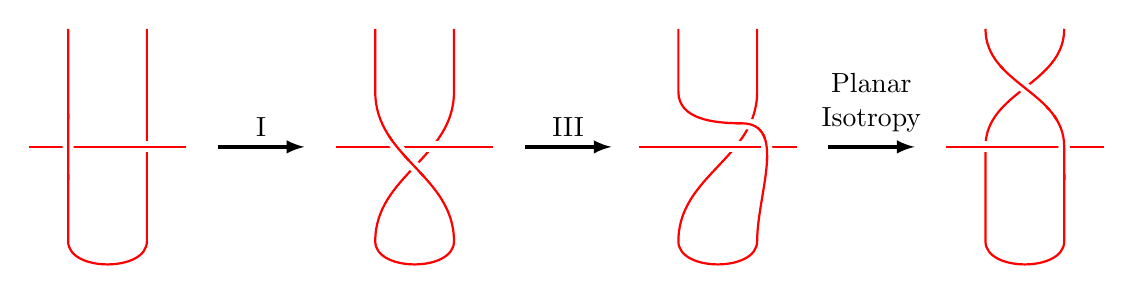
\begin{tikzpicture}
            \begin{knot}[
                xshift=-1.95cm,
                every strand/.append style={red,thick},
                clip width=5
            ]
                \strand (-0.5,1.5)
                    to (-0.5,-1.2)
                    to [out=-90,in=-90] (0.5,-1.2)
                    to (0.5,1.5)
                ;
                \strand (-1,0) to (1,0);
                \flipcrossings{2}
            \end{knot}
            \draw[very thick,-latex] (-0.55,0) -- node[above]{I} (0.55,0);
            \begin{knot}[
                xshift=1.95cm,
                every strand/.append style={red,thick},
                clip width=5,
                clip radius=3pt,
                consider self intersections
            ]
                \strand (-0.5,1.5)
                    to (-0.5,0.7)
                    to [out=-90,in=90] (0.5,-1.2)
                    to [out=-90,in=-90] (-0.5,-1.2)
                    to [out=90,in=-90] (0.5,0.7)
                    to (0.5,1.5)
                ;
                \strand (-1,0) to (1,0);
                \flipcrossings{3}
            \end{knot}
            \draw[very thick,-latex,xshift=3.9cm] (-0.55,0) -- node[above]{III} (0.55,0);
            \begin{knot}[
                xshift=5.8cm,
                every strand/.append style={red,thick},
                clip width=5,
                clip radius=3pt,
                consider self intersections,
                ignore endpoint intersections=false
            ]
                \strand (-0.5,1.5)
                    to (-0.5,0.7)
                    to [out=-90,in=180] (0.3,0.3)
                    to [out=0,in=90] (0.5,-1.2)
                    to [out=-90,in=-90] (-0.5,-1.2)
                    to [out=90,in=-90] (0.5,0.7)
                    to (0.5,1.5)
                ;
                \strand (-1,0) to (1,0);
                \flipcrossings{3}
            \end{knot}
            \draw[very thick,-latex,xshift=7.75cm] (-0.55,0) -- node[above]{
                \begin{tabular}{c}
                    Planar\\
                    Isotropy
                \end{tabular}
            } (0.55,0);
            \begin{knot}[
                xshift=9.7cm,
                every strand/.append style={red,thick},
                clip width=5,
                consider self intersections,
                ignore endpoint intersections=false
            ]
                \strand (-0.5,1.5)
                    to [out=-90,in=90] (0.5,0)
                    to (0.5,-1.2)
                    to [out=-90,in=-90] (-0.5,-1.2)
                    to (-0.5,0)
                    to [out=90,in=-90] (0.5,1.5)
                ;
                \strand (-1,0) to (1,0);
                \flipcrossings{4,5}
            \end{knot}
        \end{tikzpicture}
        \caption{Type I bridging move.}
        \label{fig:reidembridgea}
    \end{subfigure}\\
    \vspace{1em}
    \begin{subfigure}[b]{\linewidth}
        \centering
        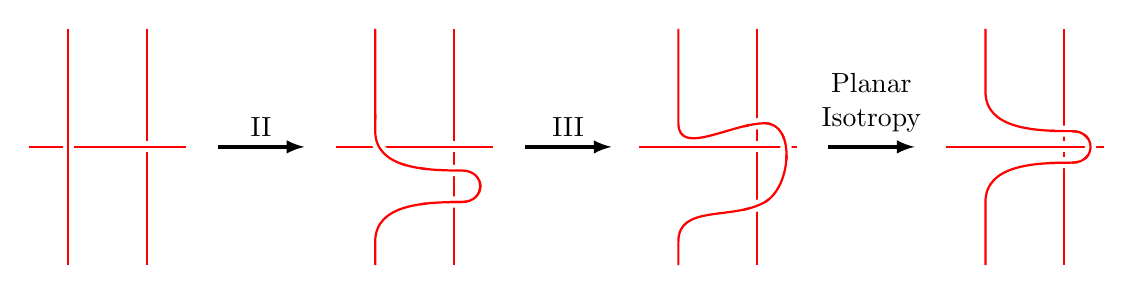
\begin{tikzpicture}
            \begin{knot}[
                xshift=-1.95cm,
                every strand/.append style={red,thick},
                clip width=5
            ]
                \strand (-0.5,-1.5) to (-0.5,1.5);
                \strand (0.5,-1.5) to (0.5,1.5);
                \strand (-1,0) to (1,0);
                \flipcrossings{2}
            \end{knot}
            \draw[very thick,-latex] (-0.55,0) -- node[above]{II} (0.55,0);
            \begin{knot}[
                xshift=1.95cm,
                every strand/.append style={red,thick},
                clip width=5,
                ignore endpoint intersections=false
            ]
                \strand (-0.5,-1.5)
                    to (-0.5,-1.2)
                    to [out=90,in=180] (0.6,-0.7)
                    to [out=0,in=0,looseness=2] (0.6,-0.3)
                    to [out=180,in=-90] (-0.5,0.2)
                    to (-0.5,1.5)
                ;
                \strand (0.5,-1.5) to (0.5,1.5);
                \strand (-1,0) to (1,0);
                \flipcrossings{4}
            \end{knot}
            \draw[very thick,-latex,xshift=3.9cm] (-0.55,0) -- node[above]{III} (0.55,0);
            \begin{knot}[
                xshift=5.8cm,
                every strand/.append style={red,thick},
                clip width=5,
                clip radius=3pt,
                ignore endpoint intersections=false
            ]
                \strand (-0.5,-1.5)
                    to (-0.5,-1.2)
                    to [out=90,in=-150] (0.6,-0.7)
                    to [out=30,in=0] (0.6,0.3)
                    to [out=180,in=-90] (-0.5,0.3)
                    to (-0.5,1.5)
                ;
                \strand (0.5,-1.5) to (0.5,1.5);
                \strand (-1,0) to (1,0);
                \flipcrossings{4}
            \end{knot}
            \draw[very thick,-latex,xshift=7.75cm] (-0.55,0) -- node[above]{
                \begin{tabular}{c}
                    Planar\\
                    Isotropy
                \end{tabular}
            } (0.55,0);
            \begin{knot}[
                xshift=9.7cm,
                every strand/.append style={red,thick},
                clip width=5,
                clip radius=3pt,
                ignore endpoint intersections=false
            ]
                \strand (-0.5,-1.5)
                    to (-0.5,-0.7)
                    to [out=90,in=180] (0.6,-0.2)
                    to [out=0,in=0,looseness=2] (0.6,0.2)
                    to [out=180,in=-90] (-0.5,0.7)
                    to (-0.5,1.5)
                ;
                \strand (0.5,-1.5) to (0.5,1.5);
                \strand (-1,0) to (1,0);
                \flipcrossings{4}
            \end{knot}
        \end{tikzpicture}
        \caption{Type II bridging move.}
        \label{fig:reidembridgeb}
    \end{subfigure}
    \caption{The legal moves that sum to the bridging moves.}
    \label{fig:reidembridge}
\end{figure}

The sequences of Reidemeister moves in Figure \ref{fig:reidembridge} sum to the bridging moves. Therefore, the bridging moves are legal.\par
Both of the bridging moves reduce the number of bridges in a projection by combining bridges, or moving inconvenient overstrands out of the way. They are also similar in the fact that they first create (a) new crossing(s) and then use a Type III Reidemeister move to "shift" one crossing along a strand to the opposite side of another$^[$\footnote{Note that it is always before and after the Type III Reidemeister move, specifically, that the number of bridges changes.}$^]$. In fact, it's worth noting that a Type I bridging move is simply a version of a Type II bridging move applicable when two strands are concerned instead of three. In effect, given the leftmost setup in Figure \ref{fig:reidembridgea}, one could use a Type II bridging move and then a Type I Reidemeister move to arrive at the rightmost setup in Figure \ref{fig:reidembridgea}$^[$\footnote{Although Figure \ref{fig:trefoilcircle} uses a Type II bridging move and Figure \ref{fig:trefoilclr} uses a Type I bridging move, Figures \ref{fig:trefoilcircleb} and \ref{fig:trefoilclrb} are interconvertible via one Type I Reidemeister move.}$^]$. The reason for making a distinction at all is twofold. First, I find the Type I bridging move to be more intuitive than the Type II and I believe that the notion of "flipping" a loop really helps cement the idea of combining bridges by shifting the relationships between crossings. Second, the leftmost setup in Figure \ref{fig:reidembridgea} is very common in Dowker reconstructions. In that setup, Type I bridging moves lead to a "cleaner" resultant projection (one with less extraneous crossings).\par
It is important to note that the bridging moves do not \emph{always} reduce the number of bridges by one; rather, they often do$^[$\footnote{For example, recall the debacle concerning Figure \ref{fig:fig8clr}.}$^]$. This observation is key --- while the bridging moves are combinations of Reidemeister moves that often reduce the number of bridges by combining bridges or moving obstructive crossings out of the way, they must still be applied with precision and cleverness to find the minimal-bridge projection.\par
Perhaps the most significant application of the bridging moves is that they provide a way to \emph{prove} that a two-bridge knot is a two-bridge knot. Given a projection of a nontrivial knot, the bridging moves provide a speedy way to reduce the number of bridges. If only the bridging moves are used to reduce the number of bridges to two, then one has used only moves that do not alter the identity of the knot to find a minimal-bridge projection. Therefore, $b(K)=2$ for the knot. However, why couldn't the knot still have $b(K)=1$? In response to this question, consider the last theorem in Section \ref{sss:definitions}, which, in proving that $b(K)\geq 2$ for a nontrivial knot, provides 2 as a lower bound on the bridge number of a nontrivial knot. Therefore, if a reduction using the bridging moves proves that $b(K)\leq 2$ for the nontrivial knot and the aforementioned theorem proves that $b(K)\geq 2$ for the nontrivial knot, $b(K)\leq 2 \cup b(K)\geq 2\Rightarrow b(K)=2$.


\subsection{Utility and Applications}\label{sss:utility}
As evidenced by Sections \ref{ss2:trefoilreduce}, \ref{ss2:fig8reduce}, and \ref{ss2:trefoilreduce-2}, the bridging moves are powerful tools for reducing the number of bridges in a knot projection. Their utility continues into more complex examples as well without the need for further bridging moves (see \cite{bib:knotnotes}, Section 3.2, the treatment of the $5_2$ knot in \emph{Exercise 3.11}). However, their applicability even extends beyond the bounds of the two-bridge knots.\par

\begin{figure}[h!]
    \centering
    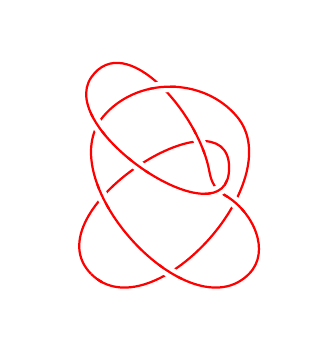
\begin{tikzpicture}[scale=0.5]
        \begin{knot}[
            clip width=5,
            clip radius=3pt,
            consider self intersections,
            ignore endpoint intersections=false
        ]
            \strand [red,thick] (-2,0)
                to [out=-45,in=-50] (1.7,4)
                to [out=130,in=50] (-1.7,4)
                to [out=-130,in=-135] (2,0)
                to [out=45,in=-30] (1.4,2)
                to [out=150,in=-80] (1,2.6)
                to [out=100,in=55] (-2,5)
                to [out=-125,in=-90,in looseness=1.2] (1.5,2.7)
                to [out=90,in=135,out looseness=1.2,in looseness=1.3] cycle
            ;
            \flipcrossings{1,4,6,8}
        \end{knot}
    \end{tikzpicture}
    \vspace{-1.5em}
    \caption{The $8_{10}$ knot.}
    \label{fig:810}
\end{figure}

In both Section \ref{sss:applications} and \ref{sss:bridging}, two-bridge knots were specifically referenced. Since they encompass all rational knots, it may seem that it would take some time to reach a prime, three-bridge knot when tabulating. Indeed it does, and $8_{10}$ is the first such knot (see Figure \ref{fig:810}). However, $8_{10}$ still displays an astonishing compatability with the techniques introduced thus far.\par

\begin{figure}[h!]
    \centering
    \begin{tikzpicture}[scale=0.5]
        \begin{knot}[
            clip width=5,
            clip radius=3pt,
            consider self intersections,
            ignore endpoint intersections=false,
            intersection 7/.append style={background color=green}
        ]
            \strand [
                red,thick,decoration={markings,
                    mark=at position 0.19 with {\arrow{>}},
                    mark=at position 0.565 with {\arrow{>}},
                    mark=at position 0.66 with {\arrow{>}},
                    mark=at position 0.84 with {\arrow{>}},
                    mark=at position 0.89 with {\arrow{>}},
                    mark=at position 0.97 with {\arrow{>}}
                },postaction={decorate}
            ]
                (-2,0)
                to [out=-45,in=-50] (1.7,4)
                to [out=130,in=50] (-1.7,4)
                to [out=-130,in=-135] (2,0)
                to [out=45,in=-30] (1.4,2)
                to [out=150,in=-80] (1,2.6)
                to [out=100,in=55] (-2,5)
                to [out=-125,in=-90,in looseness=1.2] (1.5,2.7)
                to [out=90,in=135,out looseness=1.2,in looseness=1.3] cycle
            ;
            \flipcrossings{1,4,6,8}
        \end{knot}
    \end{tikzpicture}
    \vspace{-1.5em}
    \caption{The $8_{10}$ knot being labeled in Dowker notation.}
    \label{fig:810Dowker}
\end{figure}

\begin{table}[h!]
    \centering
    \begin{tabular}{cccccccc}
        12 & 13 & 16 & 9 & 10 & 11 & 14 & 15\\
        1  & 2  & 3  & 4 & 5  & 6  & 7  & 8
    \end{tabular}
    \caption{Dowker pairs for the $8_{10}$ knot.}
    \label{tab:810Dowker}
\end{table}

While $8_{10}$ appears scary at first, its superior killzone is actually ideal. Start assigning a Dowker labeling at the \textcolor{green}{light green} crossing in Figure \ref{fig:810Dowker} and continue along the given orientation. This will generate the labeling shown in Table \ref{tab:810Dowker}.\par

\begin{figure}[H]
    \centering
    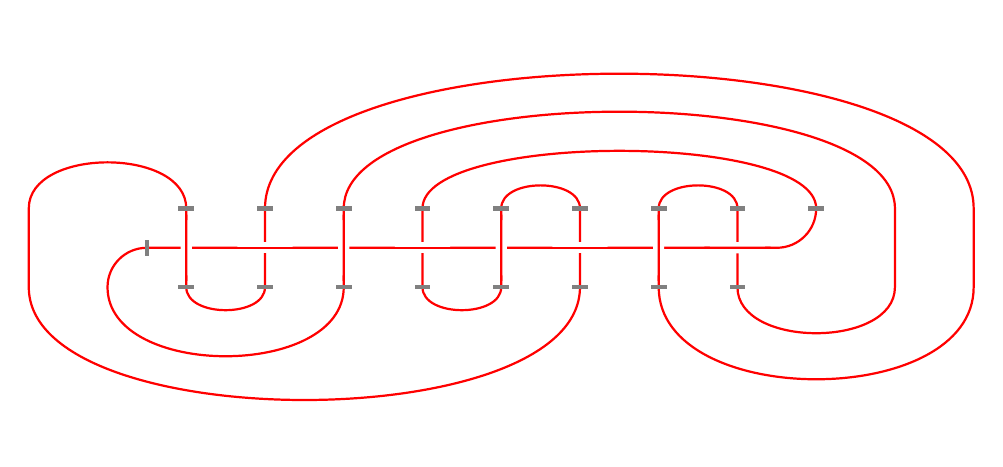
\begin{tikzpicture}
        \begin{knot}[
            clip width=5,
            consider self intersections
        ]
            \strand [red,thick] (0.5,0)
                to (8.5,0)
                to [out=0,in=-90] (9,0.5)
                to [out=90,in=90,looseness=0.5] (4,0.5)
                to (4,-0.5)
                to [out=-90,in=-90] (5,-0.5)
                to (5,0.5)
                to [out=90,in=90] (6,0.5)
                to (6,-0.5)
                to [out=-90,in=-90,looseness=0.7] (-1,-0.5)
                to (-1,0.5)
                to [out=90,in=90] (1,0.5)
                to (1,-0.5)
                to [out=-90,in=-90] (2,-0.5)
                to (2,0.5)
                to [out=90,in=90,looseness=0.65] (11,0.5)
                to (11,-0.5)
                to [out=-90,in=-90] (7,-0.5)
                to (7,0.5)
                to [out=90,in=90] (8,0.5)
                to (8,-0.5)
                to [out=-90,in=-90] (10,-0.5)
                to (10,0.5)
                to [out=90,in=90,looseness=0.6] (3,0.5)
                to (3,-0.5)
                to [out=-90,in=-90] (0,-0.5)
                to [out=90,in=180] cycle
            ;
            \flipcrossings{2,4,6,8}
        \end{knot}
        \node [verti] at (0.5,0) {};
        \node [horiz] at (9,0.5) {};
        \foreach \x in {1,...,8} {
            \foreach \y in {-0.5,0.5} {
                \node [horiz] at (\x,\y) {};
            }
        }
    \end{tikzpicture}
    \vspace{-0.8em}
    \caption{A reconstruction of the $8_{10}$ knot.}
    \label{fig:810recon}
\end{figure}

Reconstruct a knot projection from the pairings in Table \ref{tab:810Dowker} to yield Figure \ref{fig:810recon}. In this projection, there are four appealing opportunities for Type I bridging moves. However, since the middle two share a common strand, there are actually only three.\par

\begin{figure}[h!]
    \centering
    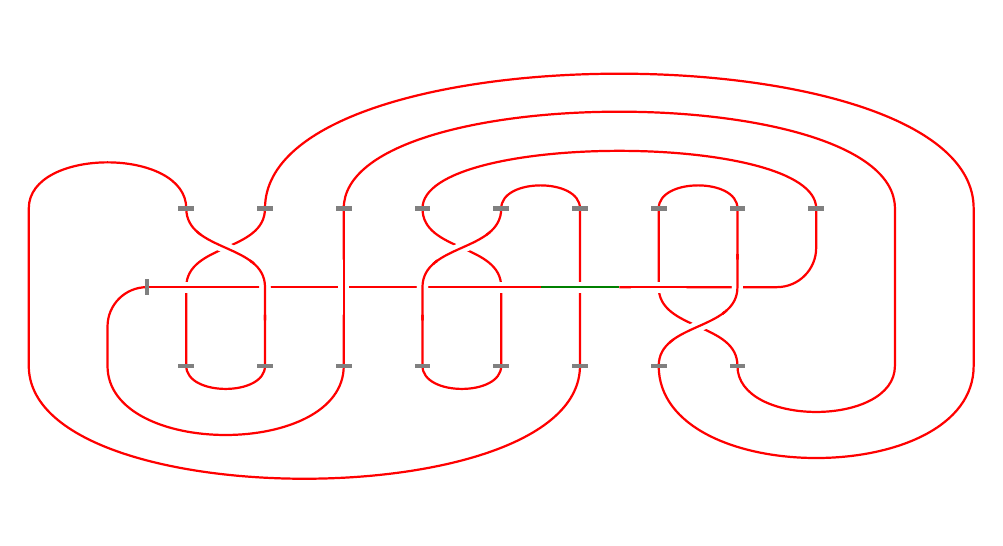
\begin{tikzpicture}
        \def\h{1}
        \begin{knot}[
            clip width=5,
            consider self intersections,
            ignore endpoint intersections=false
        ]
            \strand [red,thick] (0.5,0) to (5.5,0);
            \strand [grx,thick] (5.5,0) to (6.5,0);
            \strand [red,thick] (6.5,0)
                to (8.5,0)
                to [out=0,in=-90] (9,0.5)
                to (9,\h)
                to [out=90,in=90,looseness=0.5] (4,\h)
                to [out=-90,in=90] (5,0)
                to (5,-\h)
                to [out=-90,in=-90] (4,-\h)
                to (4,0)
                to [out=90,in=-90] (5,\h)
                to [out=90,in=90] (6,\h)
                to (6,-\h)
                to [out=-90,in=-90,looseness=0.7] (-1,-\h)
                to (-1,\h)
                to [out=90,in=90] (1,\h)
                to [out=-90,in=90] (2,0)
                to (2,-\h)
                to [out=-90,in=-90] (1,-\h)
                to (1,0)
                to [out=90,in=-90] (2,\h)
                to [out=90,in=90,looseness=0.65] (11,\h)
                to (11,-\h)
                to [out=-90,in=-90] (7,-\h)
                to [out=90,in=-90] (8,0)
                to (8,\h)
                to [out=90,in=90] (7,\h)
                to (7,0)
                to [out=-90,in=90] (8,-\h)
                to [out=-90,in=-90] (10,-\h)
                to (10,\h)
                to [out=90,in=90,looseness=0.6] (3,\h)
                to (3,-\h)
                to [out=-90,in=-90] (0,-\h)
                to (0,-0.5)
                to [out=90,in=180] (0.5,0)
            ;
            \flipcrossings{3,4,5,6,9,12,13,16}
        \end{knot}
        \node [verti] at (0.5,0) {};
        \node [horiz] at (9,\h) {};
        \foreach \x in {1,...,8} {
            \foreach \y in {-\h,\h} {
                \node [horiz] at (\x,\y) {};
            }
        }
    \end{tikzpicture}
    \vspace{-0.8em}
    \caption{Using Type I bridging moves on the $8_{10}$ knot.}
    \label{fig:810clr}
\end{figure}

To avoid an issue similar to the one associated with Figure \ref{fig:fig8clr}, choose loops that are as separated as possible. Therefore, perform three Type I bridging moves on the left, left-center, and right loops, respectively, of Figure \ref{fig:810recon} to yield Figure \ref{fig:810clr}. This new projection is already down from eight bridges to five.\par
At this point, it is time for Type II bridging moves. Of the five bridges in Figure \ref{fig:810clr}, four are two-crossing bridges and one is a three-crossing bridge. As with the figure-eight knot, it is preferable to work with a one-crossing bridge (or the bridge with the fewest number of crossings). Unfortunately, due to the four-way tie, there is no immediate front runner for which two bridges to combine. However, there exists a pair of two-crossing bridges separated by only one overpass, and every other pair of adjacent bridges is separated by at least two overpasses. Thus, with $8_{10}$ and unlike with the figure-eight knot, it is useful to consider how many overpasses separate the bridges when choosing with which one to work. Hence, the following.\par

\begin{conj}
    It is preferable to work with the bridge with the fewest overpasses separating it from the adjacent bridge.
\end{conj}

The Type II bridging move works by shifting an obstruction (a crossing of an overpass) out of the way. However, for every overpass between bridges, one Type II bridging move will be required. Therefore, the more overpasses between bridges, the more Type II bridging moves needed, and the "messier" the resultant projection.\par
Therefore, choose to move the \textcolor{grx}{green} subarc. Since it is closer to the crossings of the two-crossing bridge immediately to the left than to those of the other bridge, pull the \textcolor{grx}{green} subarc over the closer bridge. This decision will make the resultant projection "cleaner." Note, however, that the choice is ultimately arbitrary.\par

\begin{figure}[h!]
    \centering
    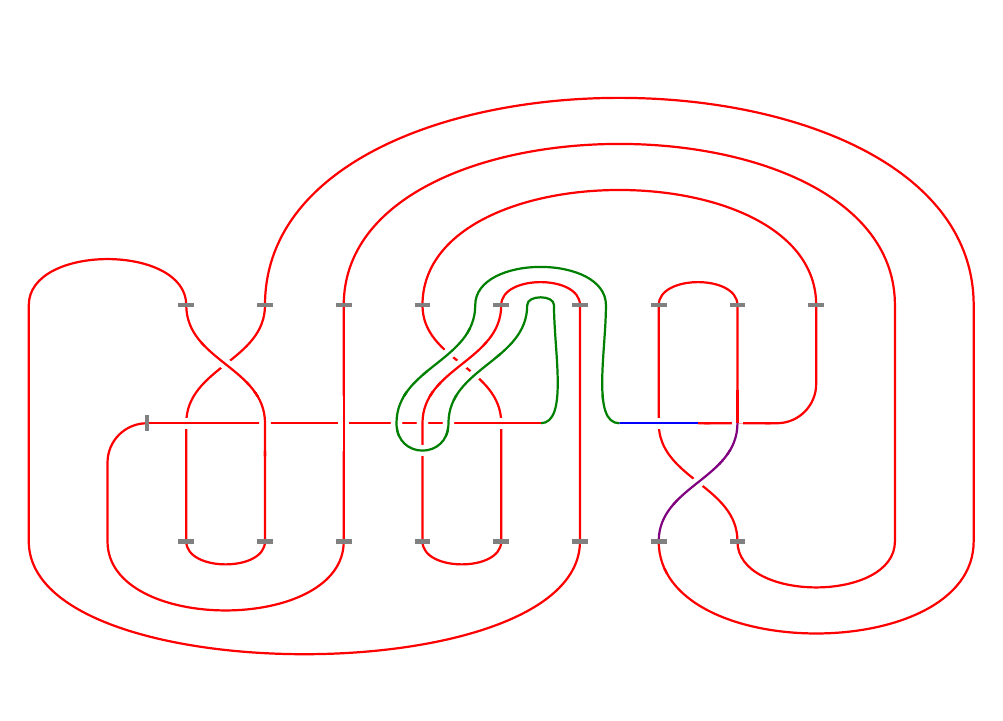
\begin{tikzpicture}
        \def\h{1.5}
        \begin{knot}[
            clip width=5,
            consider self intersections,
            ignore endpoint intersections=false
        ]
            \strand [red,thick] (0.5,0) to (5.5,0);
            \strand [grx,thick] (5.5,0)
                to [out=0,in=-90,out looseness=0.6] (5.67,\h)
                to [out=90,in=90] (5.33,\h)
                to [out=-90,in=90] (4.33,0)
                to [out=-90,in=-90,looseness=1.8] (3.67,0)
                to [out=90,in=-90] (4.67,\h)
                to [out=90,in=90] (6.33,\h)
                to [out=-90,in=180,in looseness=0.6] (6.5,0)
            ;
            \strand [blue,thick] (6.5,0) to (7.5,0);
            \strand [red,thick] (7.5,0)
                to (8.5,0)
                to [out=0,in=-90] (9,0.5)
                to (9,\h)
                to [out=90,in=90] (4,\h)
                to [out=-90,in=90] (5,0)
                to (5,-\h)
                to [out=-90,in=-90] (4,-\h)
                to (4,0)
                to [out=90,in=-90] (5,\h)
                to [out=90,in=90] (6,\h)
                to (6,-\h)
                to [out=-90,in=-90,looseness=0.7] (-1,-\h)
                to (-1,\h)
                to [out=90,in=90] (1,\h)
                to [out=-90,in=90] (2,0)
                to (2,-\h)
                to [out=-90,in=-90] (1,-\h)
                to (1,0)
                to [out=90,in=-90] (2,\h)
                to [out=90,in=90] (11,\h)
                to (11,-\h)
                to [out=-90,in=-90] (7,-\h)
            ;
            \strand [pux,thick] (7,-\h) to [out=90,in=-90] (8,0);
            \strand [red,thick] (8,0)
                to (8,\h)
                to [out=90,in=90] (7,\h)
                to (7,0)
                to [out=-90,in=90] (8,-\h)
                to [out=-90,in=-90] (10,-\h)
                to (10,\h)
                to [out=90,in=90] (3,\h)
                to (3,-\h)
                to [out=-90,in=-90] (0,-\h)
                to (0,-0.5)
                to [out=90,in=180] (0.5,0)
            ;
            \flipcrossings{2,3,4,5,8,9,10,11,14,23,24}
        \end{knot}
        \node [verti] at (0.5,0) {};
        \node [horiz] at (9,\h) {};
        \foreach \x in {1,...,8} {
            \foreach \y in {-\h,\h} {
                \node [horiz] at (\x,\y) {};
            }
        }
    \end{tikzpicture}
    \vspace{-0.8em}
    \caption{Using Type II bridging moves on the $8_{10}$ knot.}
    \label{fig:810clr-2}
\end{figure}

Perform two Type II bridging moves on the \textcolor{grx}{green} strand to yield Figure \ref{fig:810clr-2}. Note that although these contortions may not resemble a Type II bridging move, they still are --- a Type II bridging move can be thought of as pulling a crossing along a \emph{twisting} path, not just a linear one.\par
Additionally, consider why it is necessary to use \emph{two} Type II bridging moves. Should only one have been used, the two bridges would not have been combined; rather, a one-crossing bridge and another three-crossing bridge would take their place. To fully combine two bridges, it is necessary to move any obstructions \emph{all the way} out of the way.\par
Before moving on, there is another interesting occurrence in Figure \ref{fig:810clr-2}. Where the \textcolor{grx}{green} subarc exits and enters the killzone, there are no dashes. This is intentional. While the dashes have been heretofore useful solely for blocking off the killzone, in increasingly complex examples such as $8_{10}$, they become more useful as consistent reference points between figures. Although the connections may change dramatically, the killzone dashes provide a consistent frame of reference that allows even a final projection to be firmly rooted in the original.\par
At this point, the knot projection (Figure \ref{fig:810clr-2}) is down to four bridges: two two-crossing bridges, one four-crossing bridge, and one seven-crossing bridge. Choose to move the \textcolor{blue}{blue} \emph{and} \textcolor{pux}{purple} subarcs of Figure \ref{fig:810clr-2} because they are the overpasses separating the two two-crossing bridges.\par
The idea of moving two strands with two synchronized Type II bridging moves is a new one. In fact, it warrants its own definition.\par

\begin{figure}[H]
    \centering
    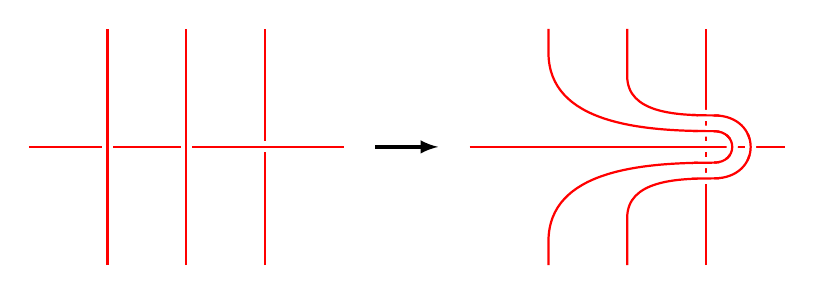
\begin{tikzpicture}
        \draw[very thick,-latex] (-0.4,0) -- (0.4,0);
        \begin{knot}[
            xshift=-2.3cm,
            every strand/.append style={red,thick},
            clip width=5
        ]
            \strand (-1.5,-1.5) to (-1.5,1.5);
            \strand (-0.5,-1.5) to (-0.5,1.5);
            \strand (0.5,-1.5) to (0.5,1.5);
            \strand (-2.5,0) to (1.5,0);
            \flipcrossings{3}
        \end{knot}
        \begin{knot}[
            xshift=3.3cm,
            every strand/.append style={red,thick},
            clip width=5,
            clip radius=3pt,
            ignore endpoint intersections=false
        ]
            \strand (-1.5,-1.5)
                to (-1.5,-1.2)
                to [out=90,in=180] (0.6,-0.2)
                to [out=0,in=0,looseness=2] (0.6,0.2)
                to [out=180,in=-90] (-1.5,1.2)
                to (-1.5,1.5)
            ;
            \strand (-0.5,-1.5)
                to (-0.5,-0.9)
                to [out=90,in=180] (0.6,-0.4)
                to [out=0,in=0,looseness=2] (0.6,0.4)
                to [out=180,in=-90] (-0.5,0.9)
                to (-0.5,1.5)
            ;
            \strand (0.5,-1.5) to (0.5,1.5);
            \strand (-2.5,0) to (1.5,0);
            \flipcrossings{7}
        \end{knot}
    \end{tikzpicture}
    \caption{A 2-set.}
    \label{fig:set}
\end{figure}

\begin{defi}
    \begin{description}
        \item[\emph{n}-Set \textnormal{(of bridging moves)}] \hfill \\ Where $n\geq 2$, $n$ Type II bridging moves that shift $n$ adjacent overpasses to the opposite side of the same crossing.
    \end{description}
\end{defi}

In knots of increasing complexity, $n$-sets become critical tools for reducing the number of bridges. The need for them arises here from the fact that in Figure \ref{fig:810clr-2}, no bridge has fewer than two overpasses separating it from its nearest neighbor.\par

\begin{figure}[h!]
    \centering
    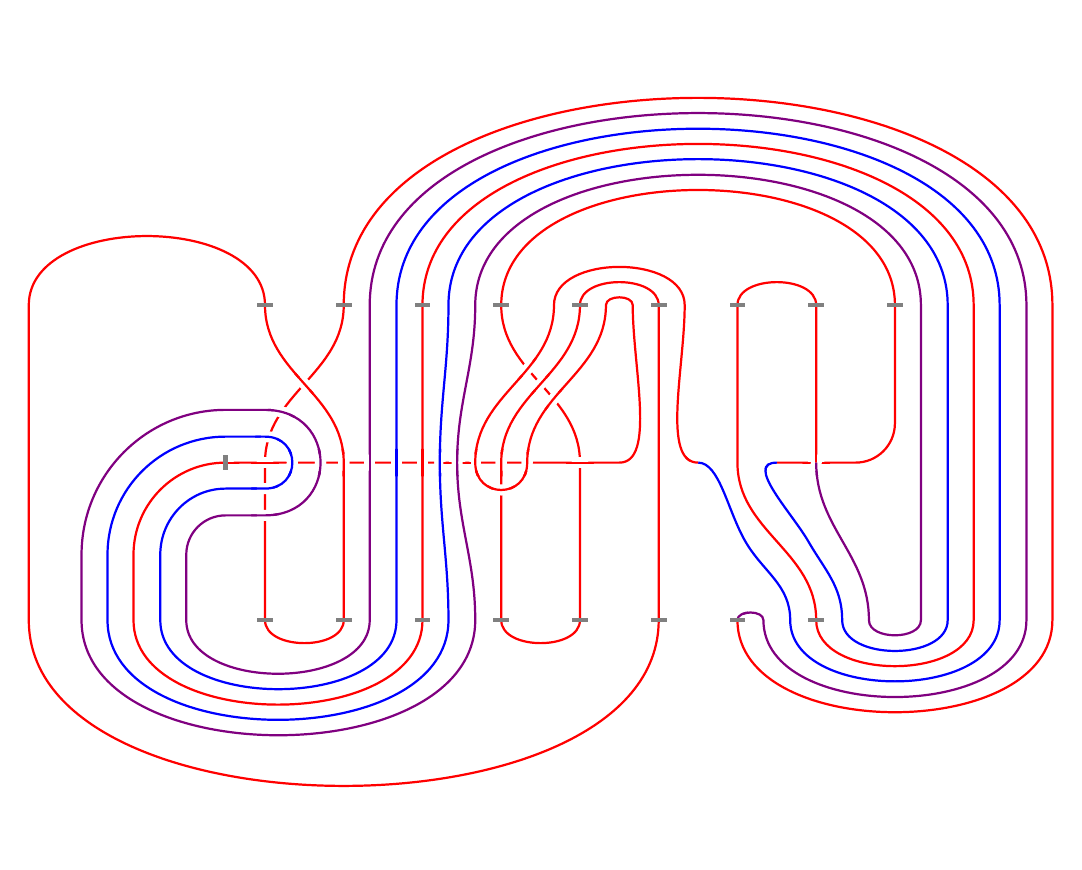
\begin{tikzpicture}
        \def\h{2}
        \begin{knot}[
            clip width=5,
            clip radius=3pt,
            consider self intersections,
            ignore endpoint intersections=false
        ]
            \strand [red,thick] (0.5,0)
                to (5.5,0)
                to [out=0,in=-90,out looseness=0.6] (5.67,\h)
                to [out=90,in=90] (5.33,\h)
                to [out=-90,in=90] (4.33,0)
                to [out=-90,in=-90,looseness=1.8] (3.67,0)
                to [out=90,in=-90] (4.67,\h)
                to [out=90,in=90] (6.33,\h)
                to [out=-90,in=180,in looseness=0.6] (6.5,0)
            ;
            \strand [blue,thick] (6.5,0)
                to [out=0,in=120,out looseness=0.6] (7.1,{-0.5*\h})
                to [out=-60,in=90] (7.67,-\h)
                to [out=-90,in=-90] (10.33,-\h)
                to (10.33,\h)
                to [out=90,in=90] (2.67,\h)
                to (2.67,-\h)
                to [out=-90,in=-90] (-0.33,-\h)
                to (-0.33,-1.17)
                to [out=90,in=180] (0.5,-0.33)
                to (1,-0.33)
                to [out=0,in=0,looseness=1.8] (1,0.33)
                to (0.5,0.33)
                to [out=180,in=90] (-1,-1.17)
                to (-1,-\h)
                to [out=-90,in=-90] (3.33,-\h)
                to [out=90,in=-90] (3.22,0)
                to [out=90,in=-90] (3.33,\h)
                to [out=90,in=90] (9.67,\h)
                to (9.67,-\h)
                to [out=-90,in=-90] (8.33,-\h)
                to [out=90,in=-60] (7.9,{-0.5*\h})
                to [out=120,in=180] (7.5,0)
            ;
            \strand [red,thick] (7.5,0)
                to (8.5,0)
                to [out=0,in=-90] (9,0.5)
                to (9,\h)
                to [out=90,in=90] (4,\h)
                to [out=-90,in=90] (5,0)
                to (5,-\h)
                to [out=-90,in=-90] (4,-\h)
                to (4,0)
                to [out=90,in=-90] (5,\h)
                to [out=90,in=90] (6,\h)
                to (6,-\h)
                to [out=-90,in=-90,looseness=0.9] (-2,-\h)
                to (-2,\h)
                to [out=90,in=90] (1,\h)
                to [out=-90,in=90] (2,0)
                to (2,-\h)
                to [out=-90,in=-90] (1,-\h)
                to (1,0)
                to [out=90,in=-90] (2,\h)
                to [out=90,in=90] (11,\h)
                to (11,-\h)
                to [out=-90,in=-90] (7,-\h)
            ;
            \strand [pux,thick] (7,-\h)
                to [out=90,in=90] (7.33,-\h)
                to [out=-90,in=-90] (10.67,-\h)
                to (10.67,\h)
                to [out=90,in=90] (2.33,\h)
                to (2.33,-\h)
                to [out=-90,in=-90] (0,-\h)
                to (0,-1.17)
                to [out=90,in=180] (0.5,-0.67)
                to (1,-0.67)
                to [out=0,in=0,looseness=1.8] (1,0.67)
                to (0.5,0.67)
                to [out=180,in=90] (-1.33,-1.17)
                to (-1.33,-\h)
                to [out=-90,in=-90] (3.67,-\h)
                to [out=90,in=-90] (3.44,0)
                to [out=90,in=-90] (3.67,\h)
                to [out=90,in=90] (9.33,\h)
                to (9.33,-\h)
                to [out=-90,in=-90] (8.67,-\h)
                to [out=90,in=-90] (8,0)
            ;
            \strand [red,thick] (8,0)
                to (8,\h)
                to [out=90,in=90] (7,\h)
                to (7,0)
                to [out=-90,in=90] (8,-\h)
                to [out=-90,in=-90] (10,-\h)
                to (10,\h)
                to [out=90,in=90] (3,\h)
                to (3,-\h)
                to [out=-90,in=-90] (-0.67,-\h)
                to (-0.67,-1.17)
                to [out=90,in=180] (0.5,0)
            ;
            \flipcrossings{1,2,3,4,5,6,7,8,9,12,13,14,15,18,19,20,22,23,33,34,36,37,38}
        \end{knot}
        \node [verti] at (0.5,0) {};
        \node [horiz] at (9,\h) {};
        \foreach \x in {1,...,8} {
            \foreach \y in {-\h,\h} {
                \node [horiz] at (\x,\y) {};
            }
        }
    \end{tikzpicture}
    \vspace{-0.8em}
    \caption{A projection of the $8_{10}$ knot with 3 bridges.}
    \label{fig:810fin}
\end{figure}

To finish, perform two 2-sets on the \textcolor{blue}{blue} and \textcolor{pux}{purple} strands to yield Figure \ref{fig:810fin}. Because $b(8_{10})=3$, Figure \ref{fig:810fin} is a minimal-bridge projection.\par
Using three Type I bridging moves, two Type II bridging moves, and two 2-sets (seven total distinct transformations), five bridges were removed. Although Figure \ref{fig:810fin} is not in any way "clean," it is a systematically discoverable projection of $8_{10}$ with only three bridges.
\newpage



\section{Conjectures}
In the course of writing this paper, several further ideas concerning this new theory of bridging moves have arisen. As no immediately evident proof has presented itself to me, I include this section to list several related conjectures. Each will be followed by a short explanation of my current reasoning.

\begin{conj}
    Given a reduced projection of an alternating knot, sequences of Type I and Type II bridging moves suffice to find a minimal-bridge projection.
\end{conj}

Through the examples of the trefoil, figure-eight, and $8_{10}$ knots, it has become clear that the bridging moves are powerful tools for reducing the number of bridges in a projection. However, every example so far has been an alternating knot already in a minimal-crossing projection, so these are important qualifiers.\par
It may seem that this conjecture is really implying nothing --- if the bridging moves are composed of the Reidemeister moves, then isn't this conjecture arguing that the Reidemeister moves suffice to find a minimal projection? Actually, the bridging moves are specific sequences of Reidemeister moves, so this conjecture implies (for example) that a Type I Reidemeister move would never \emph{need} to be followed by a Type II Reidemeister move, a Type II Reidemeister move would never \emph{need} to be followed by a Type I Reidemeister move, etc. Perhaps the main point of this conjecture is that there would never be cause to define such a thing as a Type III bridging move.\par
Since, as was previously mentioned, a Type I bridging move is really a special case of a Type II bridging move, I present the following, bolder conjecture.

\begin{conj}
    Given a reduced projection of an alternating knot, sequences of Type II bridging moves suffice to find a minimal-bridge projection.
\end{conj}

This conjecture implies that a Type I Reidemeister move will never be necessary to find the minimal-bridge projection. Note that this conjecture still implies all that was stated above in the previous conjecture. The implication would seem to make sense, as a Type I Reidemeister move only adds or removes extraneous crossings, which would already have been removed in a minimal-crossing projection of an alternating knot. However, it cannot be immediately ruled out that the bridging moves might generate an easily removed crossing (see \cite{bib:knotnotes}, Figure 3.9) in the course of finding a minimal-bridge projection.\par
Thinking through $8_{10}$ in Section \ref{sss:utility} has led to several revelations. First, I will define my concept of being self-terminal.

\begin{figure}[h!]
    \centering
    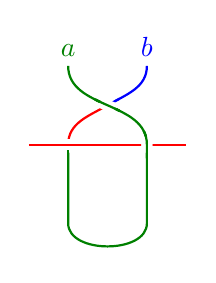
\begin{tikzpicture}
        \begin{knot}[
            every strand/.append style={thick},
            clip width=5,
            clip radius=3pt,
            consider self intersections,
            ignore endpoint intersections=false
        ]
            \strand [grx] (0,1) node[above]{$a$}
                to [out=-90,in=90] (1,0)
                to (1,-1)
                to [out=-90,in=-90] (0,-1)
                to (0,0)
            ;
            \strand [red] (0,0) 
                to [out=90,in=-150] (0.5,0.5)
            ;
            \strand [blue] (0.5,0.5)
                to [out=30,in=-90] (1,1) node[above]{$b$}
            ;
            \strand [red] (-0.5,0) to (1.5,0);
            \flipcrossings{6,7,8}
            \redraw{1}{(0.5,0.5)}
        \end{knot}
    \end{tikzpicture}
    \caption{An example of a self-terminal end.}
    \label{fig:selfter}
\end{figure}

\begin{defi}
    \begin{description}
        \item[Self-terminal \textnormal{(end)}] \hfill \\ An end of bridge $a$ such that one or more of the overpasses separating bridge $a$ from bridge $b$ are part of bridge $a$.
        \item[Self-terminal \textnormal{(bridge)}] \hfill \\ A bridge where both ends are self-terminal.
    \end{description}
\end{defi}

In Figure \ref{fig:selfter}, notice how both the \textcolor{red}{horizontal red} strand and bridge $\color{grx}a$ separate bridge $\color{grx}a$ from bridge $\color{blue}b$. Because bridge $\color{grx}a$ is one of the two separating strands, this end of bridge $\color{grx}a$ is self-terminal.\par
Self-terminality has already played an important role. In choosing which direction to move the \textcolor{blue}{blue} and \textcolor{pux}{purple} subarcs of Figure \ref{fig:810clr-2}, I suspect that I \emph{had} to move them in the direction that I did because the end on the other side of them was self-terminal. Furthermore, based on my observations of the four-crossing and seven-crossing bridges in Figure \ref{fig:810clr-2}, I conjecture the following.

\begin{conj}
    Self-terminal bridges cannot be combined with other bridges.
\end{conj}

A Type II bridging move works by shifting overpasses out of the way. If one of these overpasses is the bridge itself, then a recursive cycle has been created. As a second way of thinking about this, consider Figure \ref{fig:selfter}. While the horizontal \textcolor{red}{red} strand could be pulled down, around, and along bridge $\color{grx}a$ using a Type II bridging move, it would seem to be impossible to pull bridge $\color{grx}a$ along itself.\par
The previous conjecture has a critical corollary, which follows.

\begin{conj}
    If all bridges in a projection are self-terminal, then the projection is a minimal-bridge projection and $b(K)$ is equal to the number of bridges in that projection.
\end{conj}

If this conjecture is true, a projection such as Figure \ref{fig:810fin} (where all bridges are self-terminal) would establish definitive proof that $b(8_{10})=3$. The implications of this would be enormous since \emph{proving} that $b(K)>2$ for a knot is currently very difficult.\par
Returning to the bridging moves, I conjecture the following.

\begin{conj}
    A knot is in its minimal-bridge projection if and only if all possible bridging moves and $n$-sets change its number of bridges by $0$ or $+1$.
\end{conj}

In Figure \ref{fig:810fin}, it would appear that there are no bridging moves or $n$-sets capable of reducing the number of bridges. This would be difficult to verify, as there are many cases to consider, but I suspect that this observation should suffice as proof that $b(8_{10})=3$.\par
This conjecture may again appear insignificant, but it inextricably ties bridge number to the bridging moves by suggesting that it is only when the bridging moves have no effect that a knot is in its minimal-bridge projection. Obviously, if a knot \emph{is} in its minimal-bridge projection, the bridging moves will have no effect, but this conjecture concerns the converse of that statement.\par
I am undecided as to this last conjecture, but it would be nice if it were true. Bridging moves often add extraneous crossings and unnecessary loops. This is especially obvious in Figure \ref{fig:810fin}. To find a "cleaner" projection, these extraneous crossings can be "weeded out" of the minimal-bridge projection without increasing the number of bridges. This rather tedious process generates a "minimal-crossing minimal-bridge projection." Because of its tediousness, I conjecture the following.

\begin{conj}
    There is a simpler way to find a minimal-crossing minimal-bridge projection than by using the bridging moves and then eliminating extraneous crossings.
\end{conj}

This conjecture implies that while the bridging moves \emph{can} (as implied by the first conjecture) reduce the number of bridges to $b(K)$ and the Reidemeister moves \emph{can} then reduce the number of crossings to the fewest possible in a minimal-bridge projection, there exists some sort of hybrid method to accomplish both at the same time. Such a method would certainly be profound and would also be incredibly useful, but at least for now, the bridging moves and self-terminality are the pinnacle of my meditations.
\newpage



\bibliography{BridgeNumber}
\bibliographystyle{apalike}

\noindent All figures are my own designs, created in Ti\emph{k}Z with style influenced by \cite{bib:knotbook}. The color-coding for the definition and theorem boxes was inspired by Sheldon Axler's \emph{Linear Algebra Done Right}.




\end{document}